
\subsection{Desarrollo}
El desarrollo del incremento comenzó con la creación y configuración del proyecto en \textbf{Supabase}. En primer lugar, se definió la tabla \textbf{\textit{profiles}} \figref{fig:supabase_profiles_table}, destinada a almacenar los datos públicos de los usuarios. Cada registro de esta tabla contiene un campo \textbf{id} que actúa como clave foránea y referencia al identificador del usuario en la tabla \textbf{\textit{auth.users}}, estableciendo una relación configurada con acciones en cascada. Esto permite la actualización automática de los datos en caso de modificaciones en cualquiera de las tablas relacionadas.

Entre los atributos almacenados en la tabla \textbf{\textit{profiles}} se encuentra el \textbf{nombre de usuario}, el cual se definió como único. Dado que este valor debía establecerse durante el proceso de registro, fue necesario implementar una \textbf{función} \figref{fig:supabase_username_function} junto con un \textbf{\textit{trigger}} \figref{fig:supabase_username_trigger} que capturase el nombre de usuario almacenado en los metadatos del registro y lo persistiera en la tabla correspondiente.

Adicionalmente, se definieron las políticas \figref{fig:supabase_profiles_permissions} de \textbf{actualización de la información}, permitiendo a los usuarios autenticados modificar únicamente sus propios datos, así como las políticas de \textbf{visualización}, que habilitan el acceso de lectura a todos los usuarios sobre la información almacenada en la tabla \textbf{\textit{profiles}}.

\begin{figure}[H]
    \centering
    \begin{subfigure}[t]{0.48\textwidth}
        \centering
        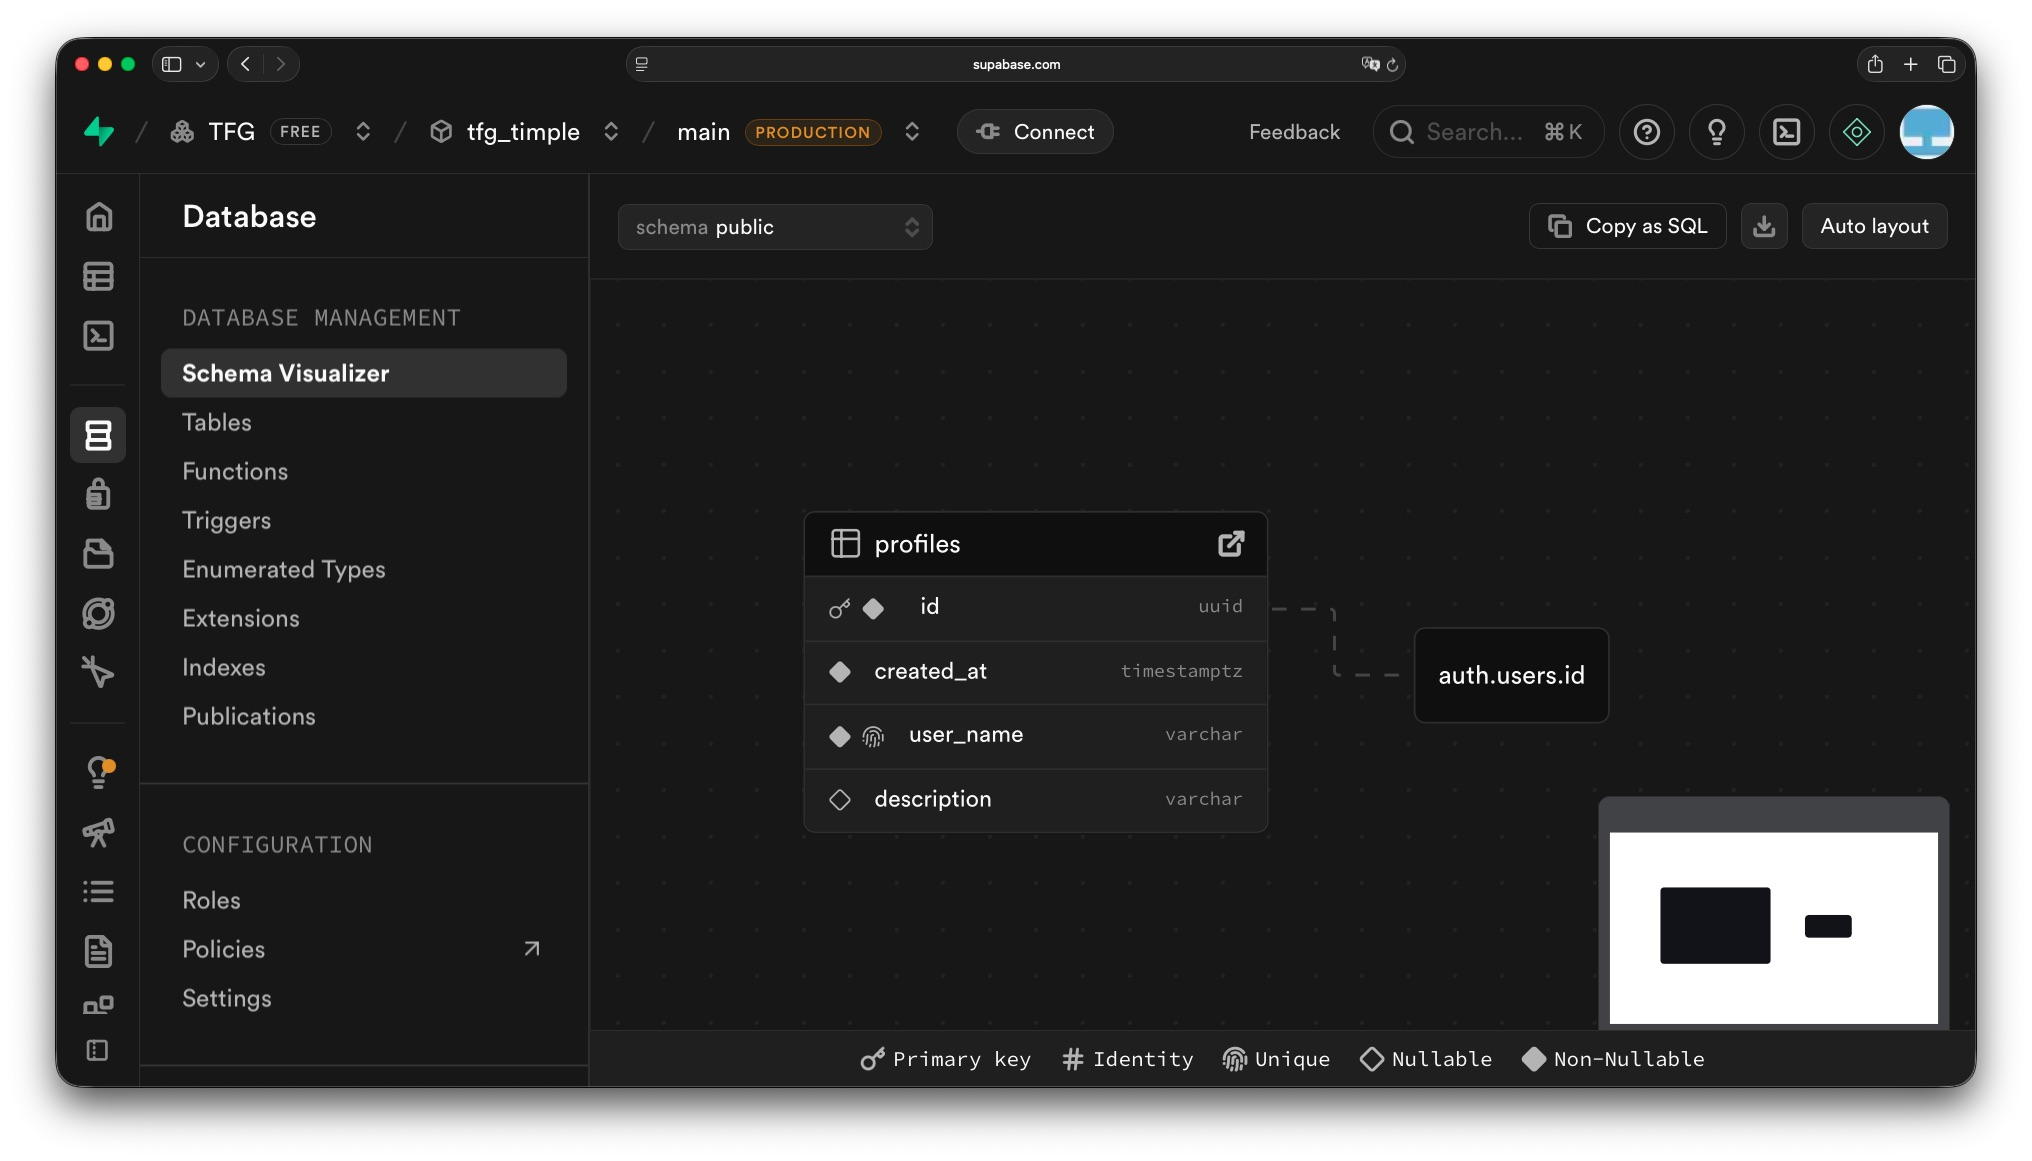
\includegraphics[width=\textwidth]{Ilustraciones/desarrollo/incremento1/desarrollo/supabase_profiles_table.jpeg}
        \caption{Tabla \textit{profiles} en Supabase}\label{fig:supabase_profiles_table}
    \end{subfigure}\hfill
    \begin{subfigure}[t]{0.48\textwidth}
        \centering
        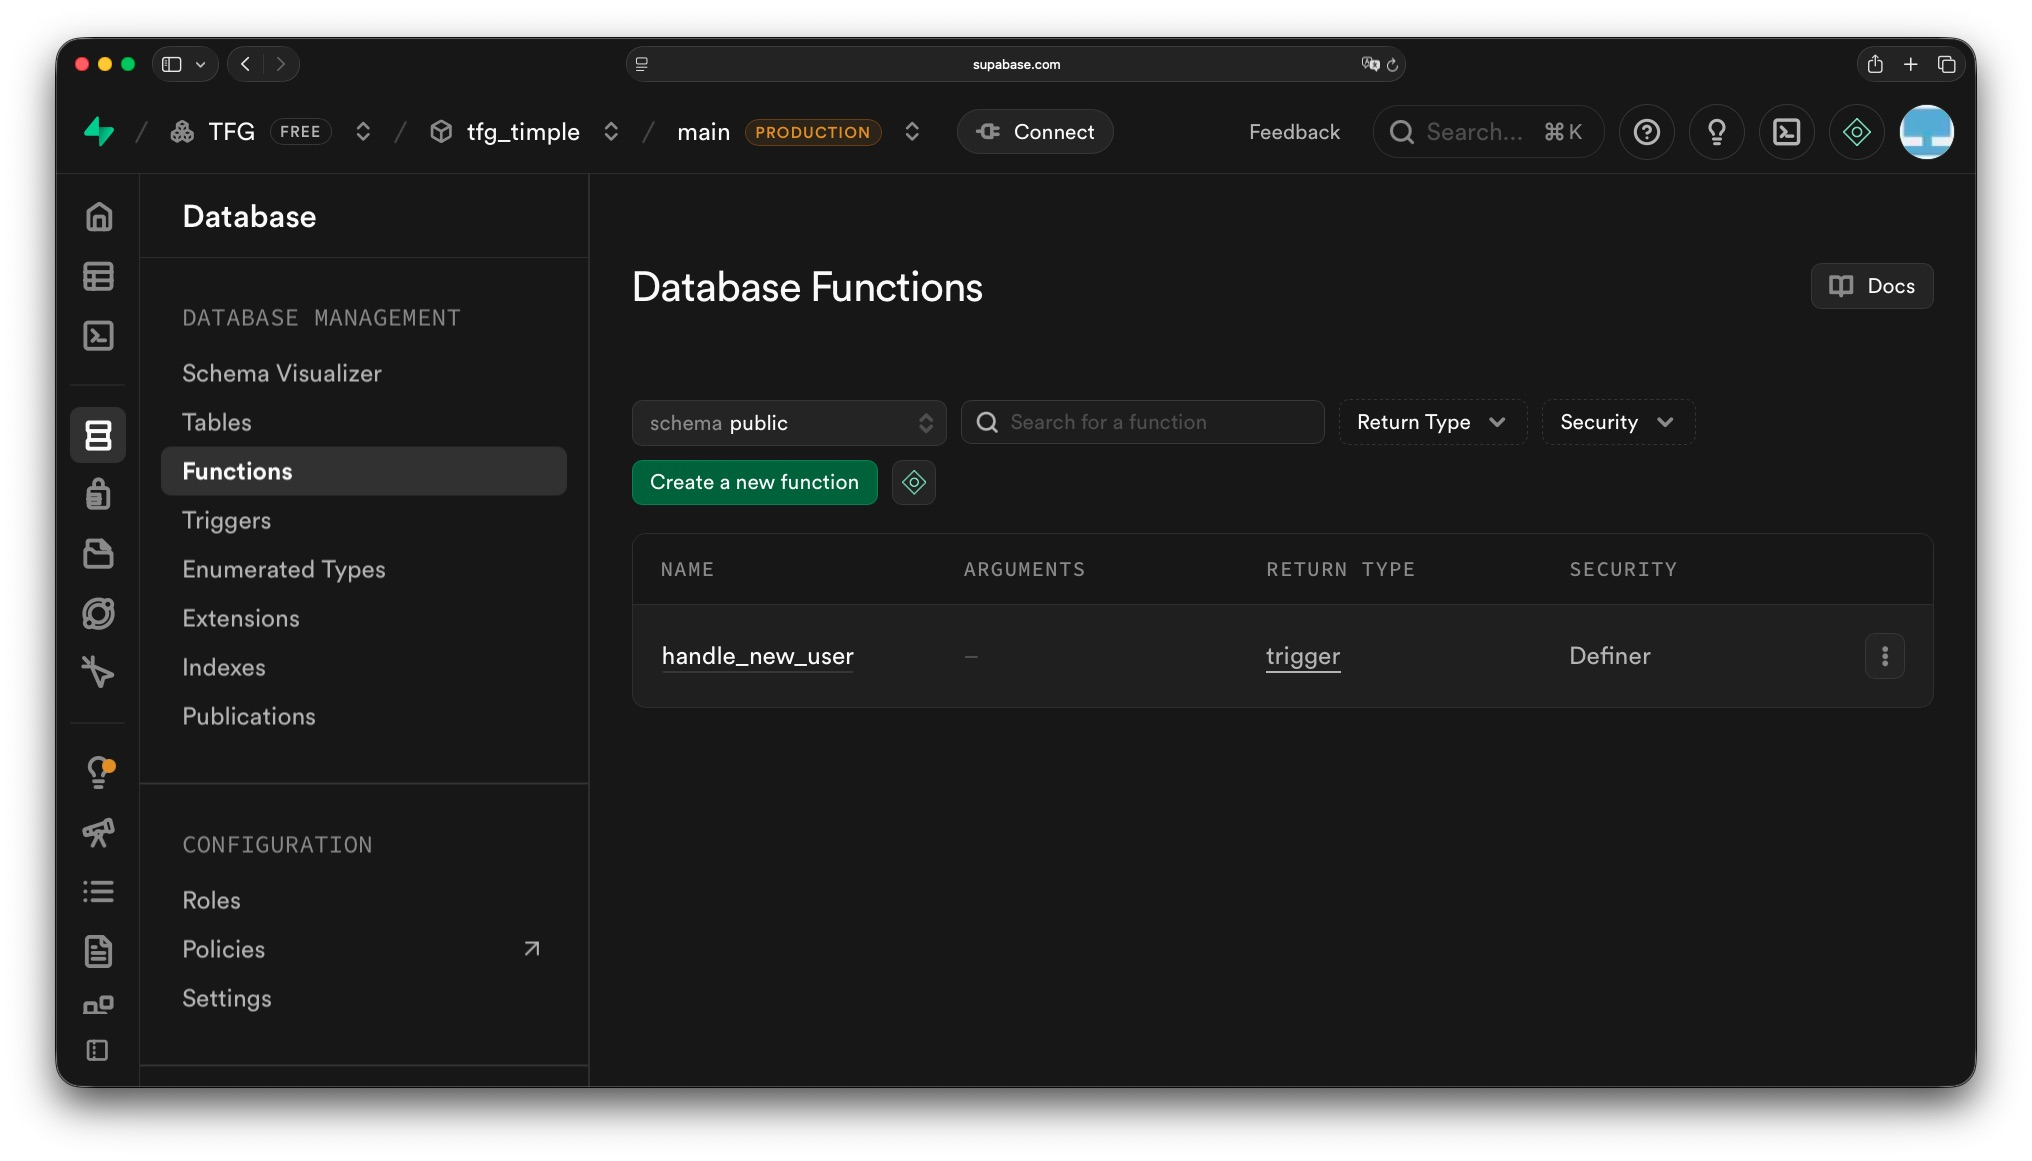
\includegraphics[width=\textwidth]{Ilustraciones/desarrollo/incremento1/desarrollo/supabase_username_function.jpeg}
        \caption{Función para la captación de nombre de usuario en los metadados}\label{fig:supabase_username_function}
    \end{subfigure}
    \vspace{1em}

    \begin{subfigure}[t]{0.48\textwidth}
        \centering
        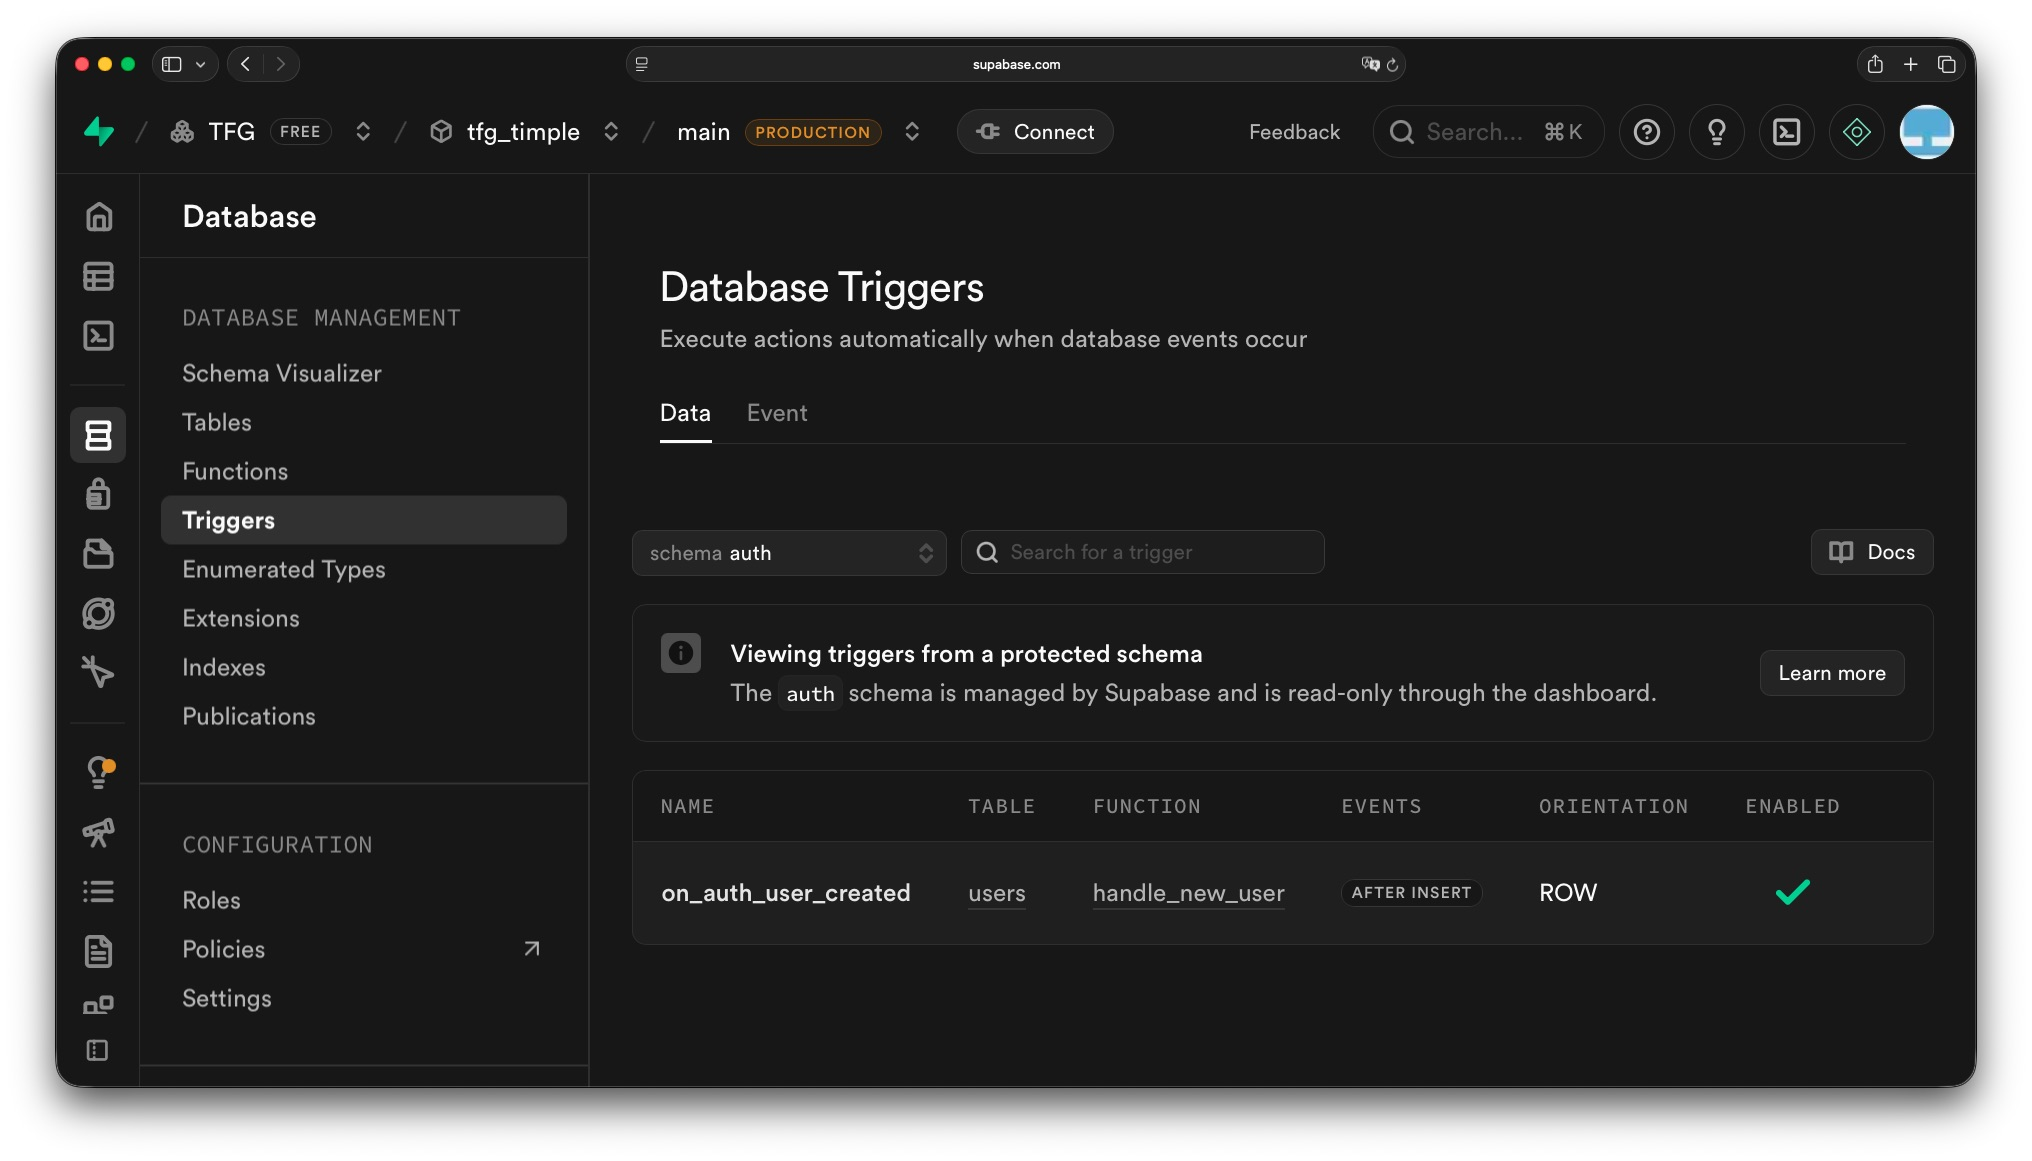
\includegraphics[width=\textwidth]{Ilustraciones/desarrollo/incremento1/desarrollo/supabase_username_trigger.jpeg}
        \caption{\textit{Trigger} con actuación tras el registro de usuario y ejecución de función de captación de nombre de usuario}\label{fig:supabase_username_trigger}
    \end{subfigure}\hfill
    \begin{subfigure}[t]{0.48\textwidth}
        \centering
        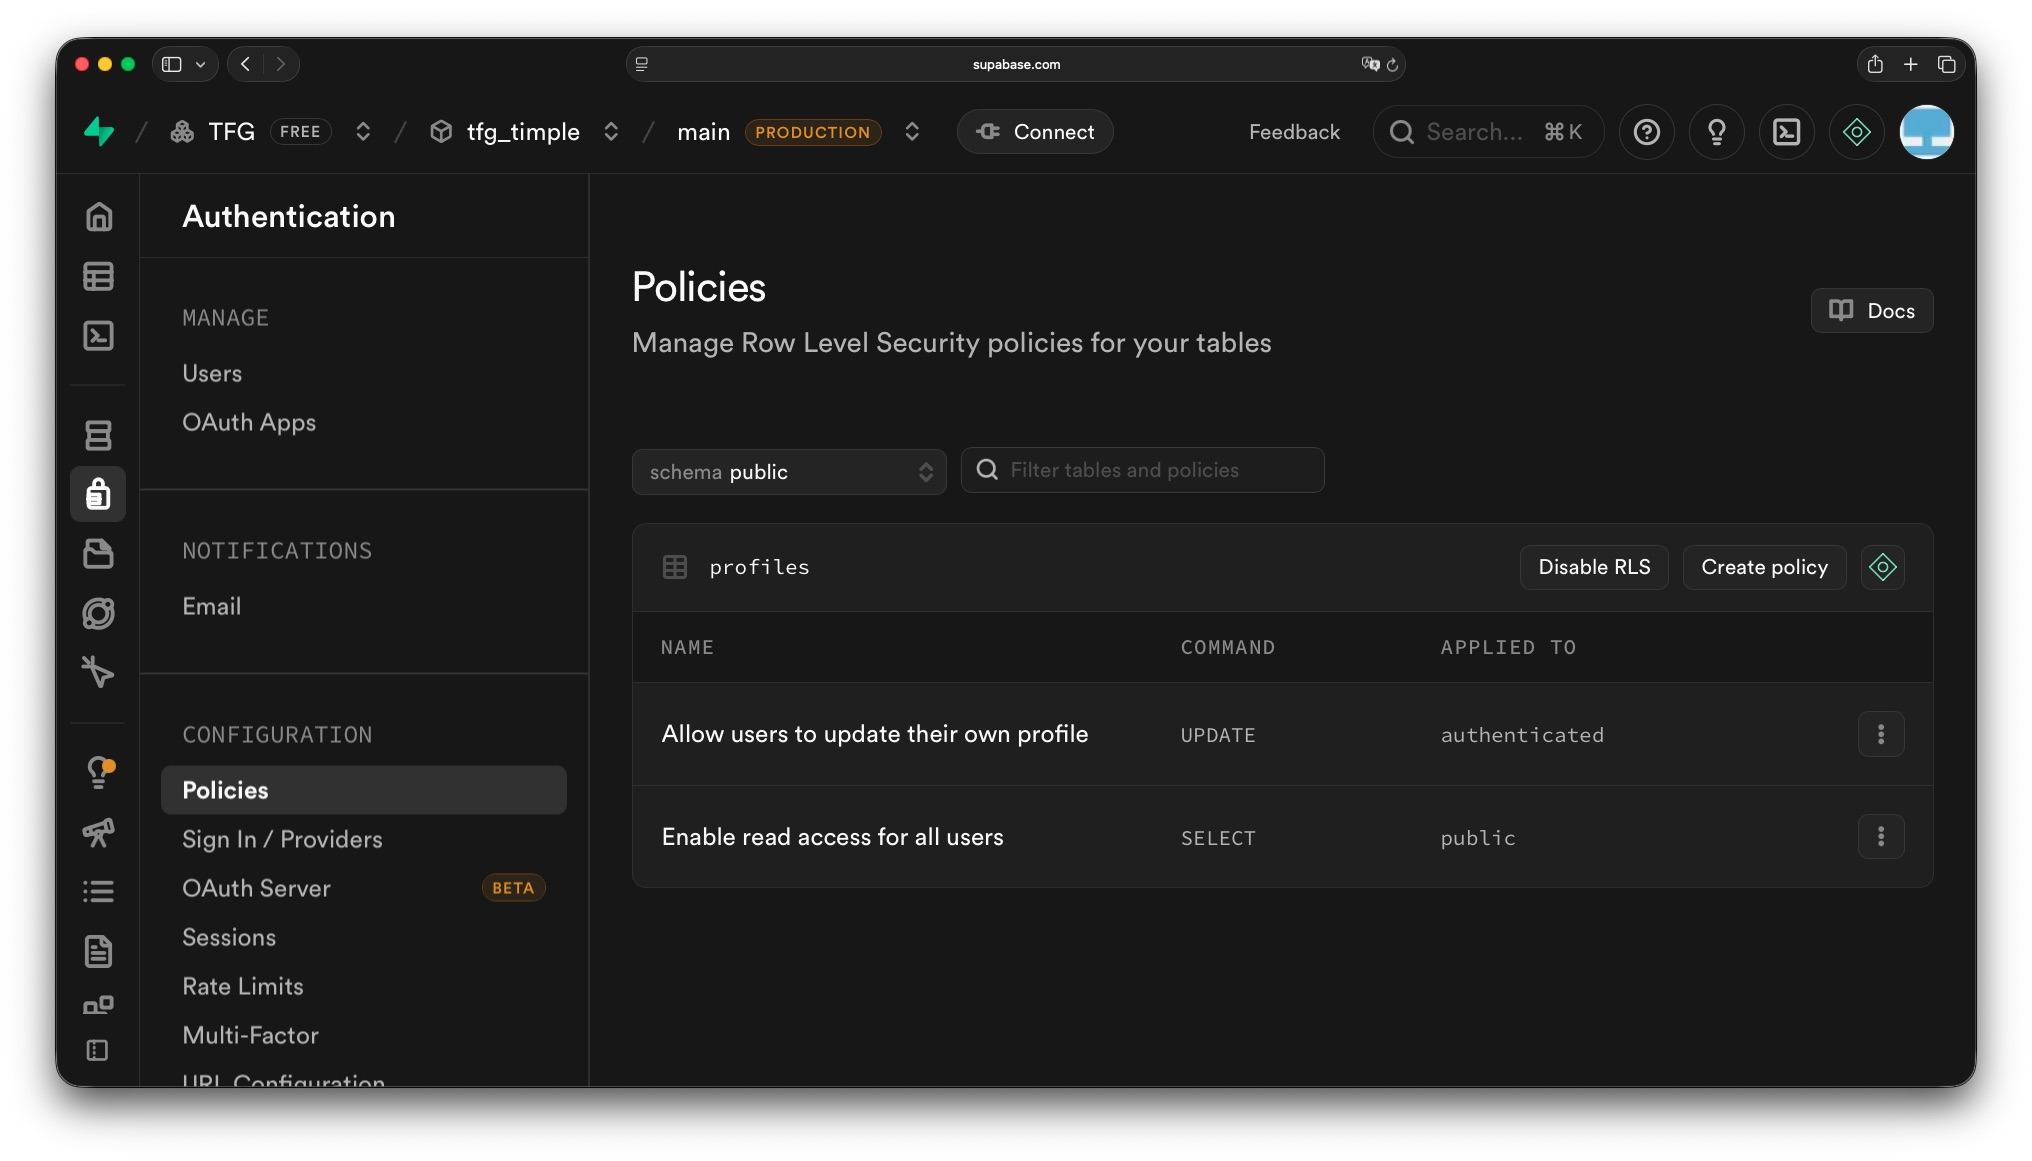
\includegraphics[width=\textwidth]{Ilustraciones/desarrollo/incremento1/desarrollo/supabase_policies.jpeg}
        \caption{Permisos de actualización y visualización de datos de la tabla \textit{profiles}}\label{fig:supabase_profiles_permissions}
    \end{subfigure}

    \caption{Creación de tabla \textit{profiles} y configuración de acciones y permisos}\label{fig:supabase_incremento_1}
\end{figure}

En segundo lugar se creó el proyecto \textbf{Next.Js} utilizando la plantilla \textbf{\textit{Next.js Supabase Auth Starter}} que incluye una configuración básica con \textbf{Supabase} y formularios de registro, inicio de sesión, cambio de contraseña y páginas públicas y privadas.

\begin{figure}[H]
    \centering
    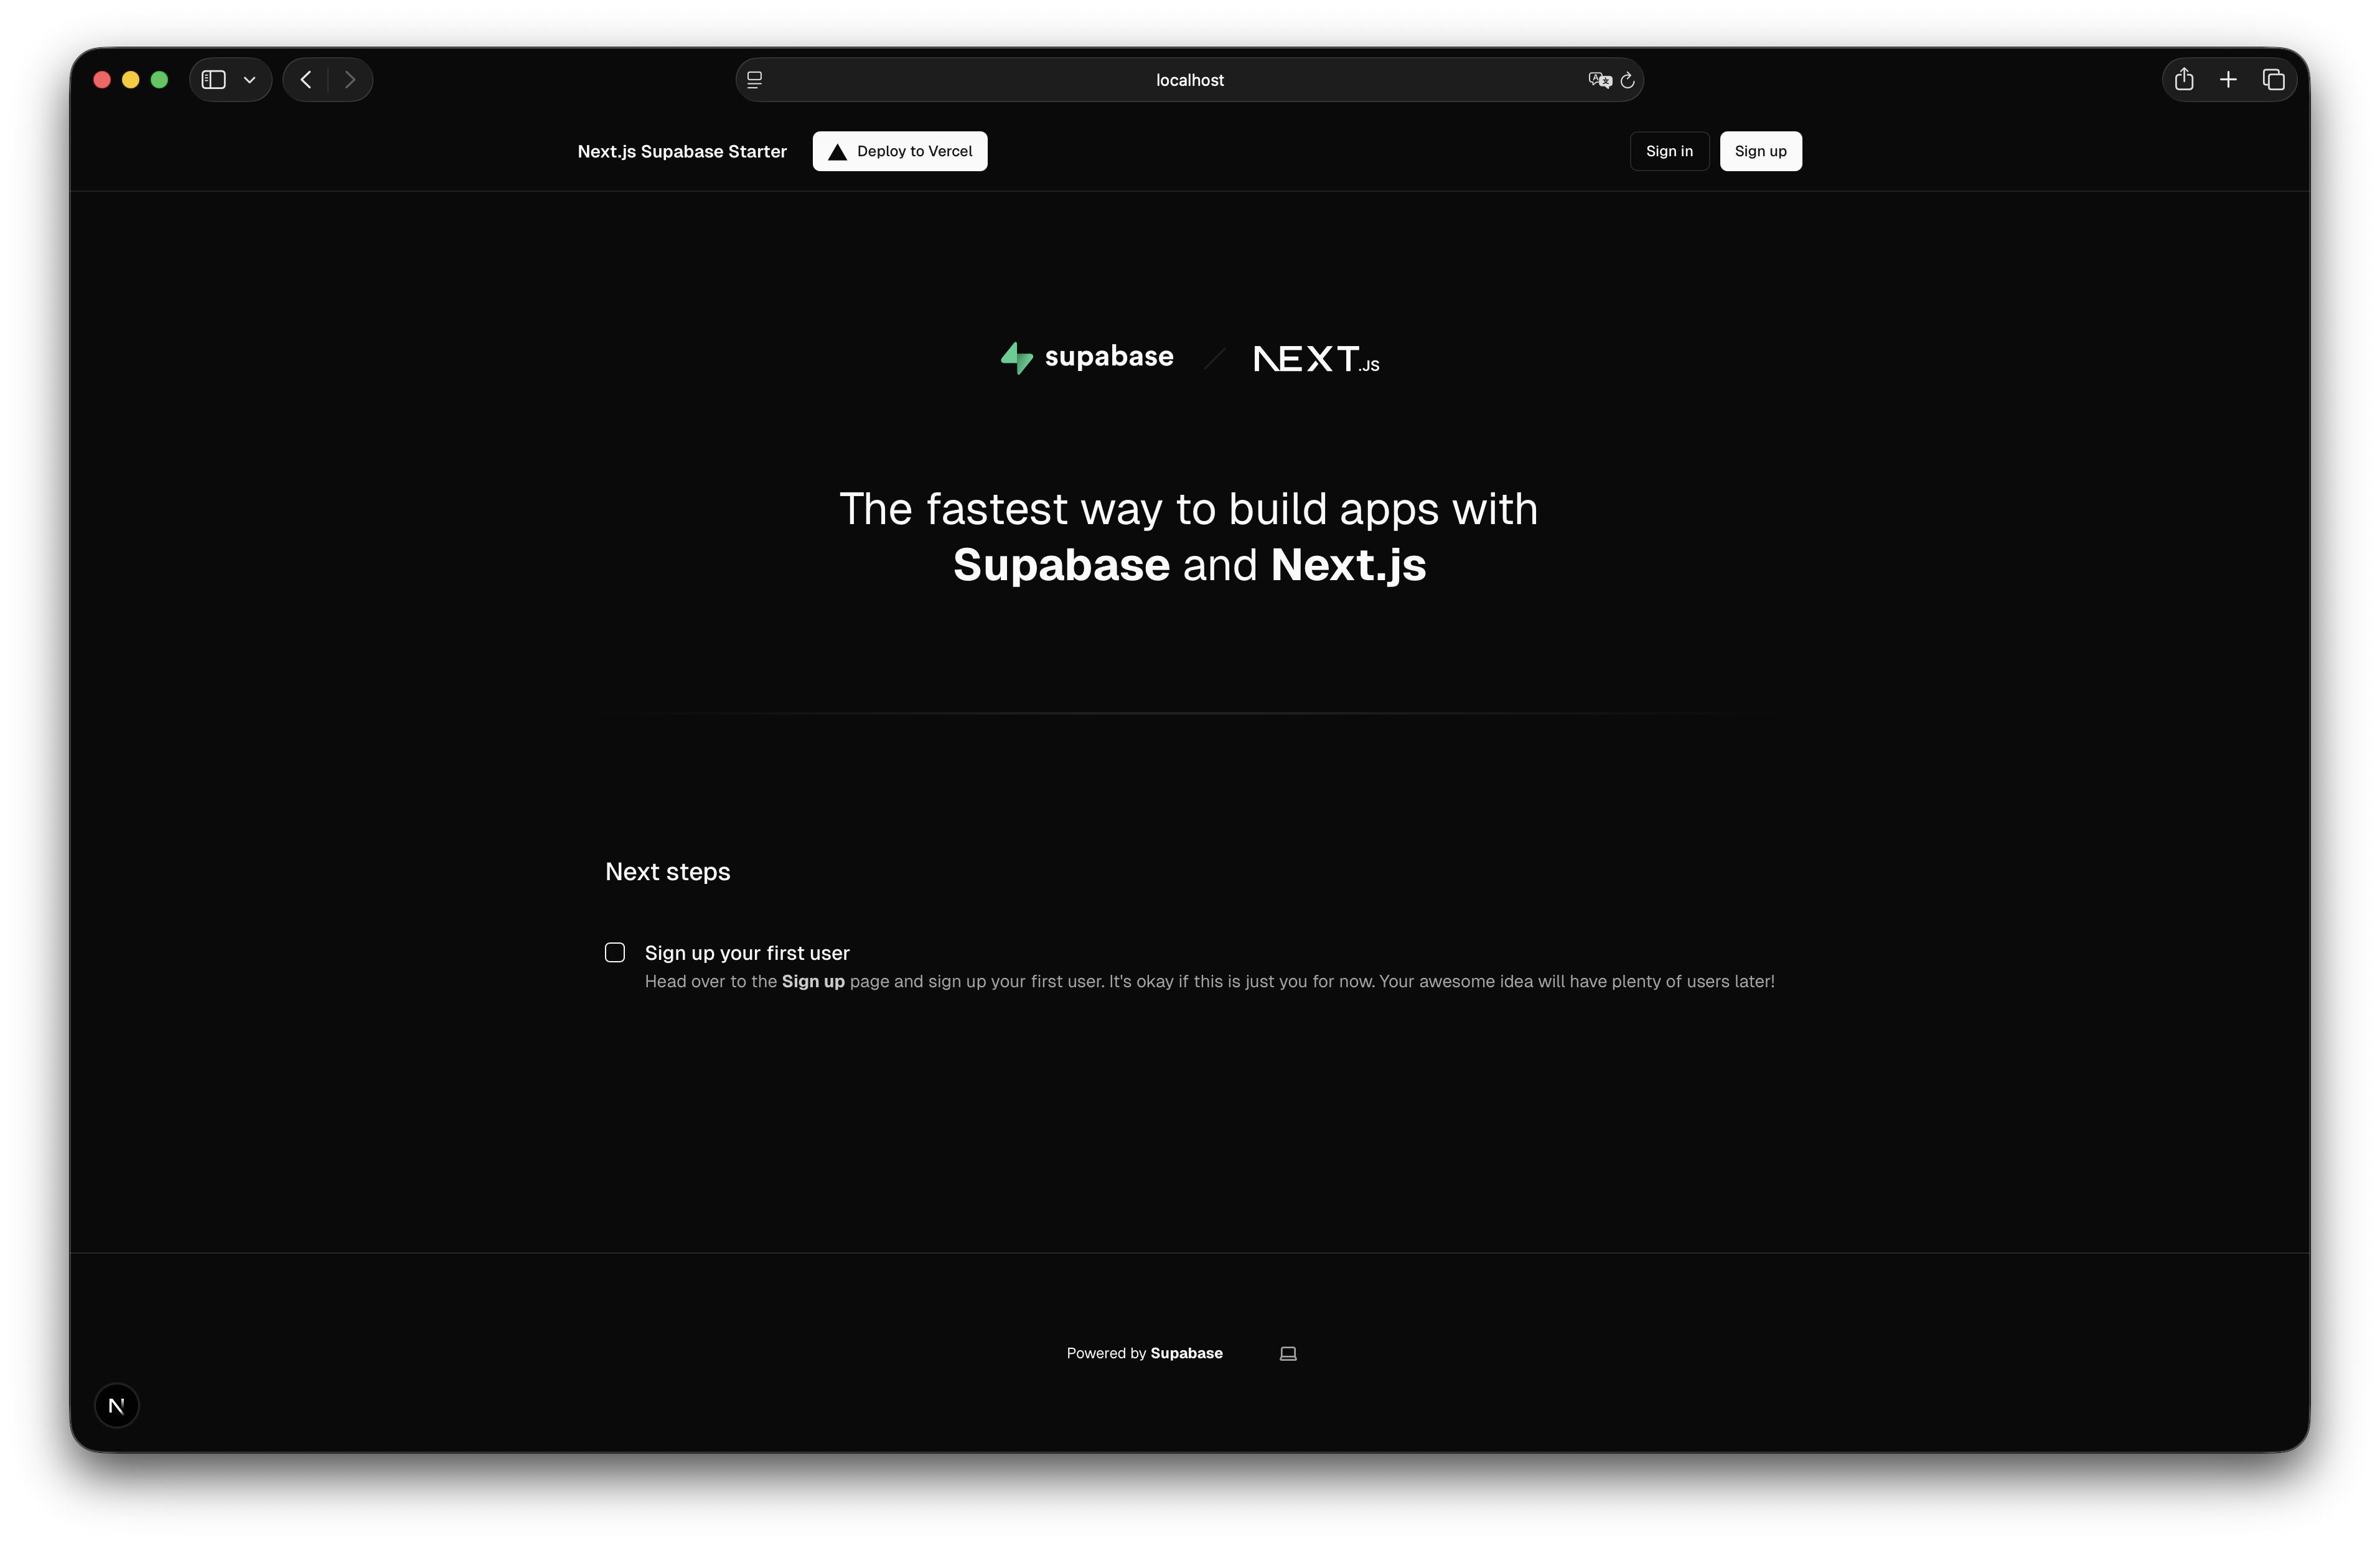
\includegraphics[width=0.8\textwidth]{Ilustraciones/desarrollo/incremento1/desarrollo/supabase_template.jpeg}    

    \caption{Plantilla de \textit{Next.js Supabase Auth Starter}}\label{fig:supabase_template}
\end{figure}

El primer cambio realizado fue de carácter visual \figref{fig:login_1}, adaptando todos los elementos ya existentes al diseño definido en el apartado anterior.

\begin{figure}[H]
    \centering
    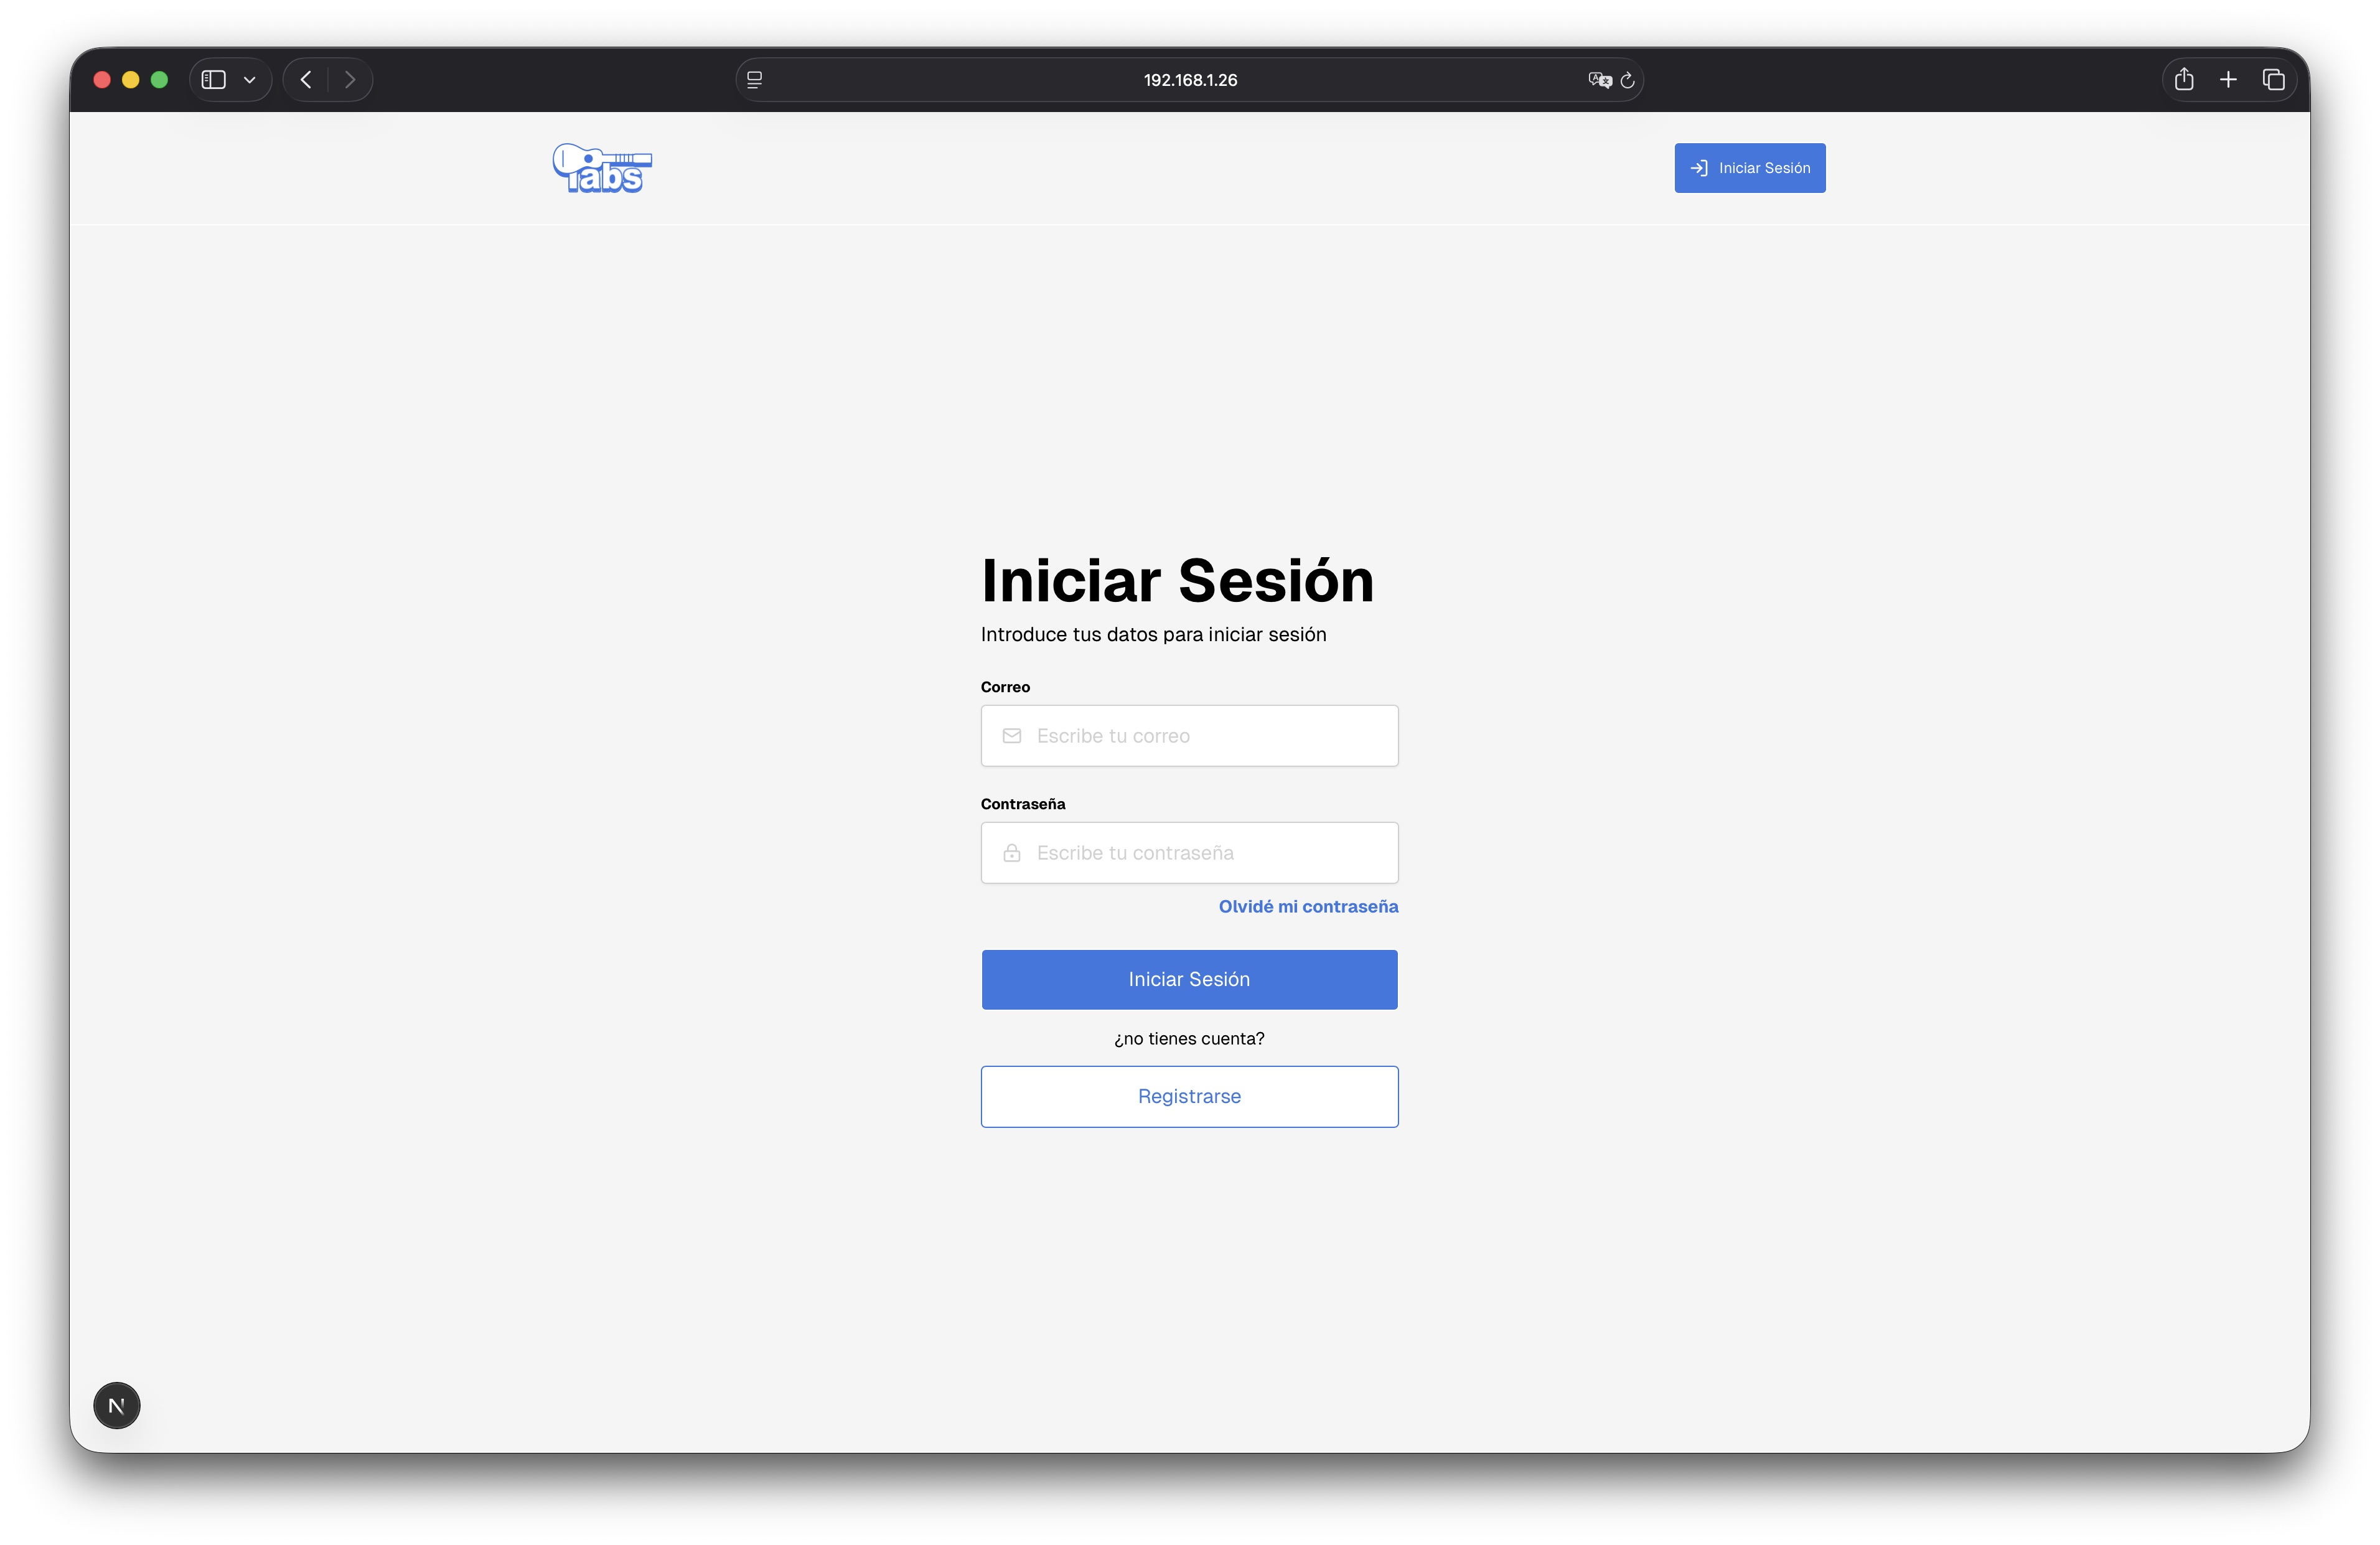
\includegraphics[width=0.8\textwidth]{Ilustraciones/desarrollo/incremento1/desarrollo/login_1.jpeg}    

    \caption{Plantilla de \textit{Next.js Supabase Auth Starter} con diseño actualizado}\label{fig:login_1}
\end{figure}

Dado que la plantilla inicial incluía las funciones de escritura y lectura de información directamente en las páginas y componentes del \textit{front-end}, el siguiente paso consistió en trasladar dichas funciones al directorio \textit{/lib} \figref{fig:lib_directories}. De este modo, se crearon las funciones de acceso y modificación de la información necesarias para el desarrollo del primer incremento.

Para estructurar este módulo, se definieron varios directorios con responsabilidades diferenciadas: \textit{actions}, destinado a acciones comunes como la validación de correo electrónico, contraseña y nombre de usuario; \textit{auth}, que contiene las funciones relacionadas con el inicio de sesión, el registro y la recuperación de contraseña; \textit{user}, con funciones específicas para usuarios autenticados, tales como la carga y modificación de información o la eliminación de la cuenta; y \textit{public}, que agrupa las funciones destinadas a usuarios no autenticados, como la carga de información pública.

Cada una de estas funciones dispone de un conjunto de pruebas unitarias \figref{fig:tests_i1} diseñadas para verificar su correcto funcionamiento.


\begin{figure}[H]
    \centering
    \begin{subfigure}[t]{0.32\textwidth}
        \centering
        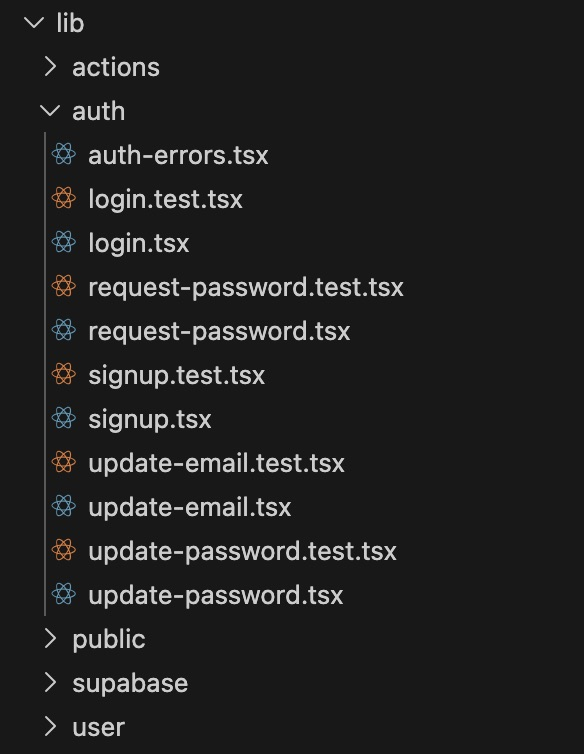
\includegraphics[width=\textwidth]{Ilustraciones/desarrollo/incremento1/desarrollo/lib_directories.jpeg}
        \caption{Directorio \textit{lib}, directorios, funciones y pruebas}\label{fig:lib_directories}
    \end{subfigure}\hfill
    \begin{subfigure}[t]{0.64\textwidth}
        \centering
        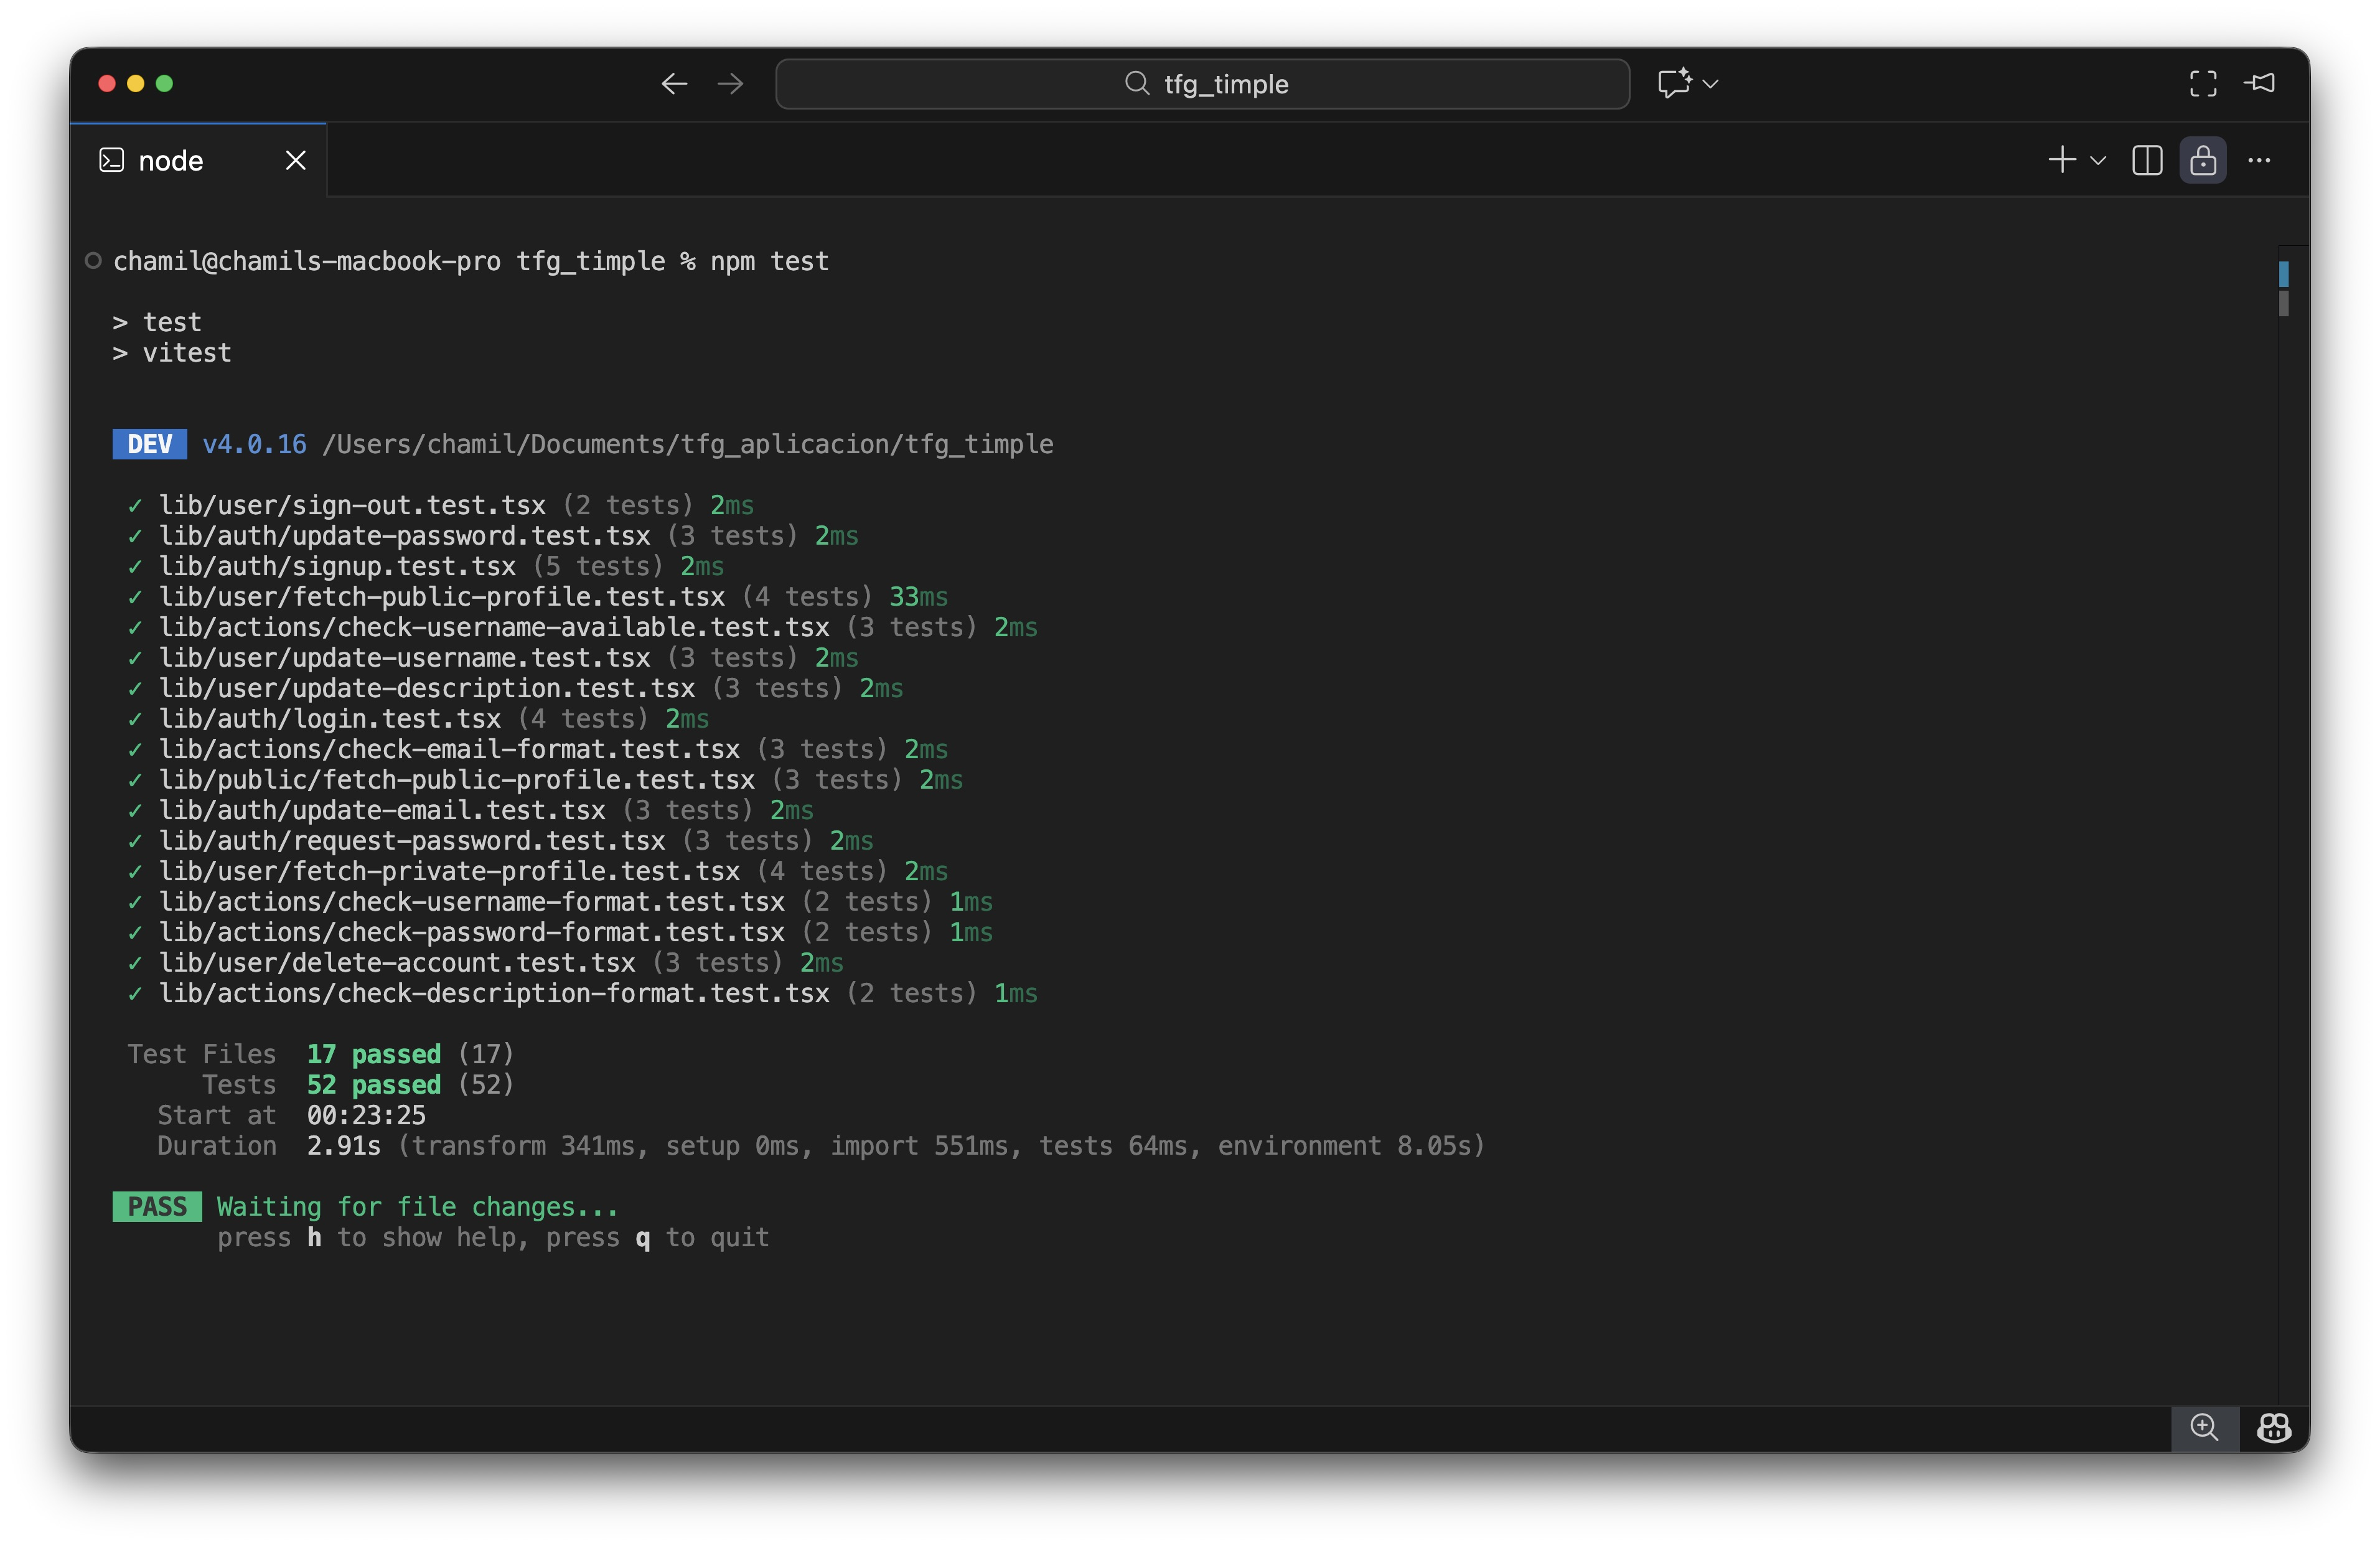
\includegraphics[width=\textwidth]{Ilustraciones/desarrollo/incremento1/desarrollo/tests_i1.jpeg}
        \caption{Ejecución de pruebas utilizando \textit{Vitest}}\label{fig:tests_i1}
    \end{subfigure}
    
    \caption{Contenidos del directorio \textit{lib} y ejecución de pruebas}\label{fig:back_end_i1}
\end{figure}

Una vez finalizada la configuración de \textbf{Supabase}, la actualización visual de la plantilla y la creación y prueba de las funciones de obtención y modificación de datos, se procedió a implementar las páginas y componentes restantes, haciendo especial mención de:

\begin{itemize}
    \item El \textbf{manual del usuario} \figref{fig:manual} y las \textbf{preguntas frecuentes}, donde se implementaron colecciones que almacenan toda la información a mostrar, facilitando la adición y modificación de contenidos.
    
    \begin{figure}[H]
        \centering
        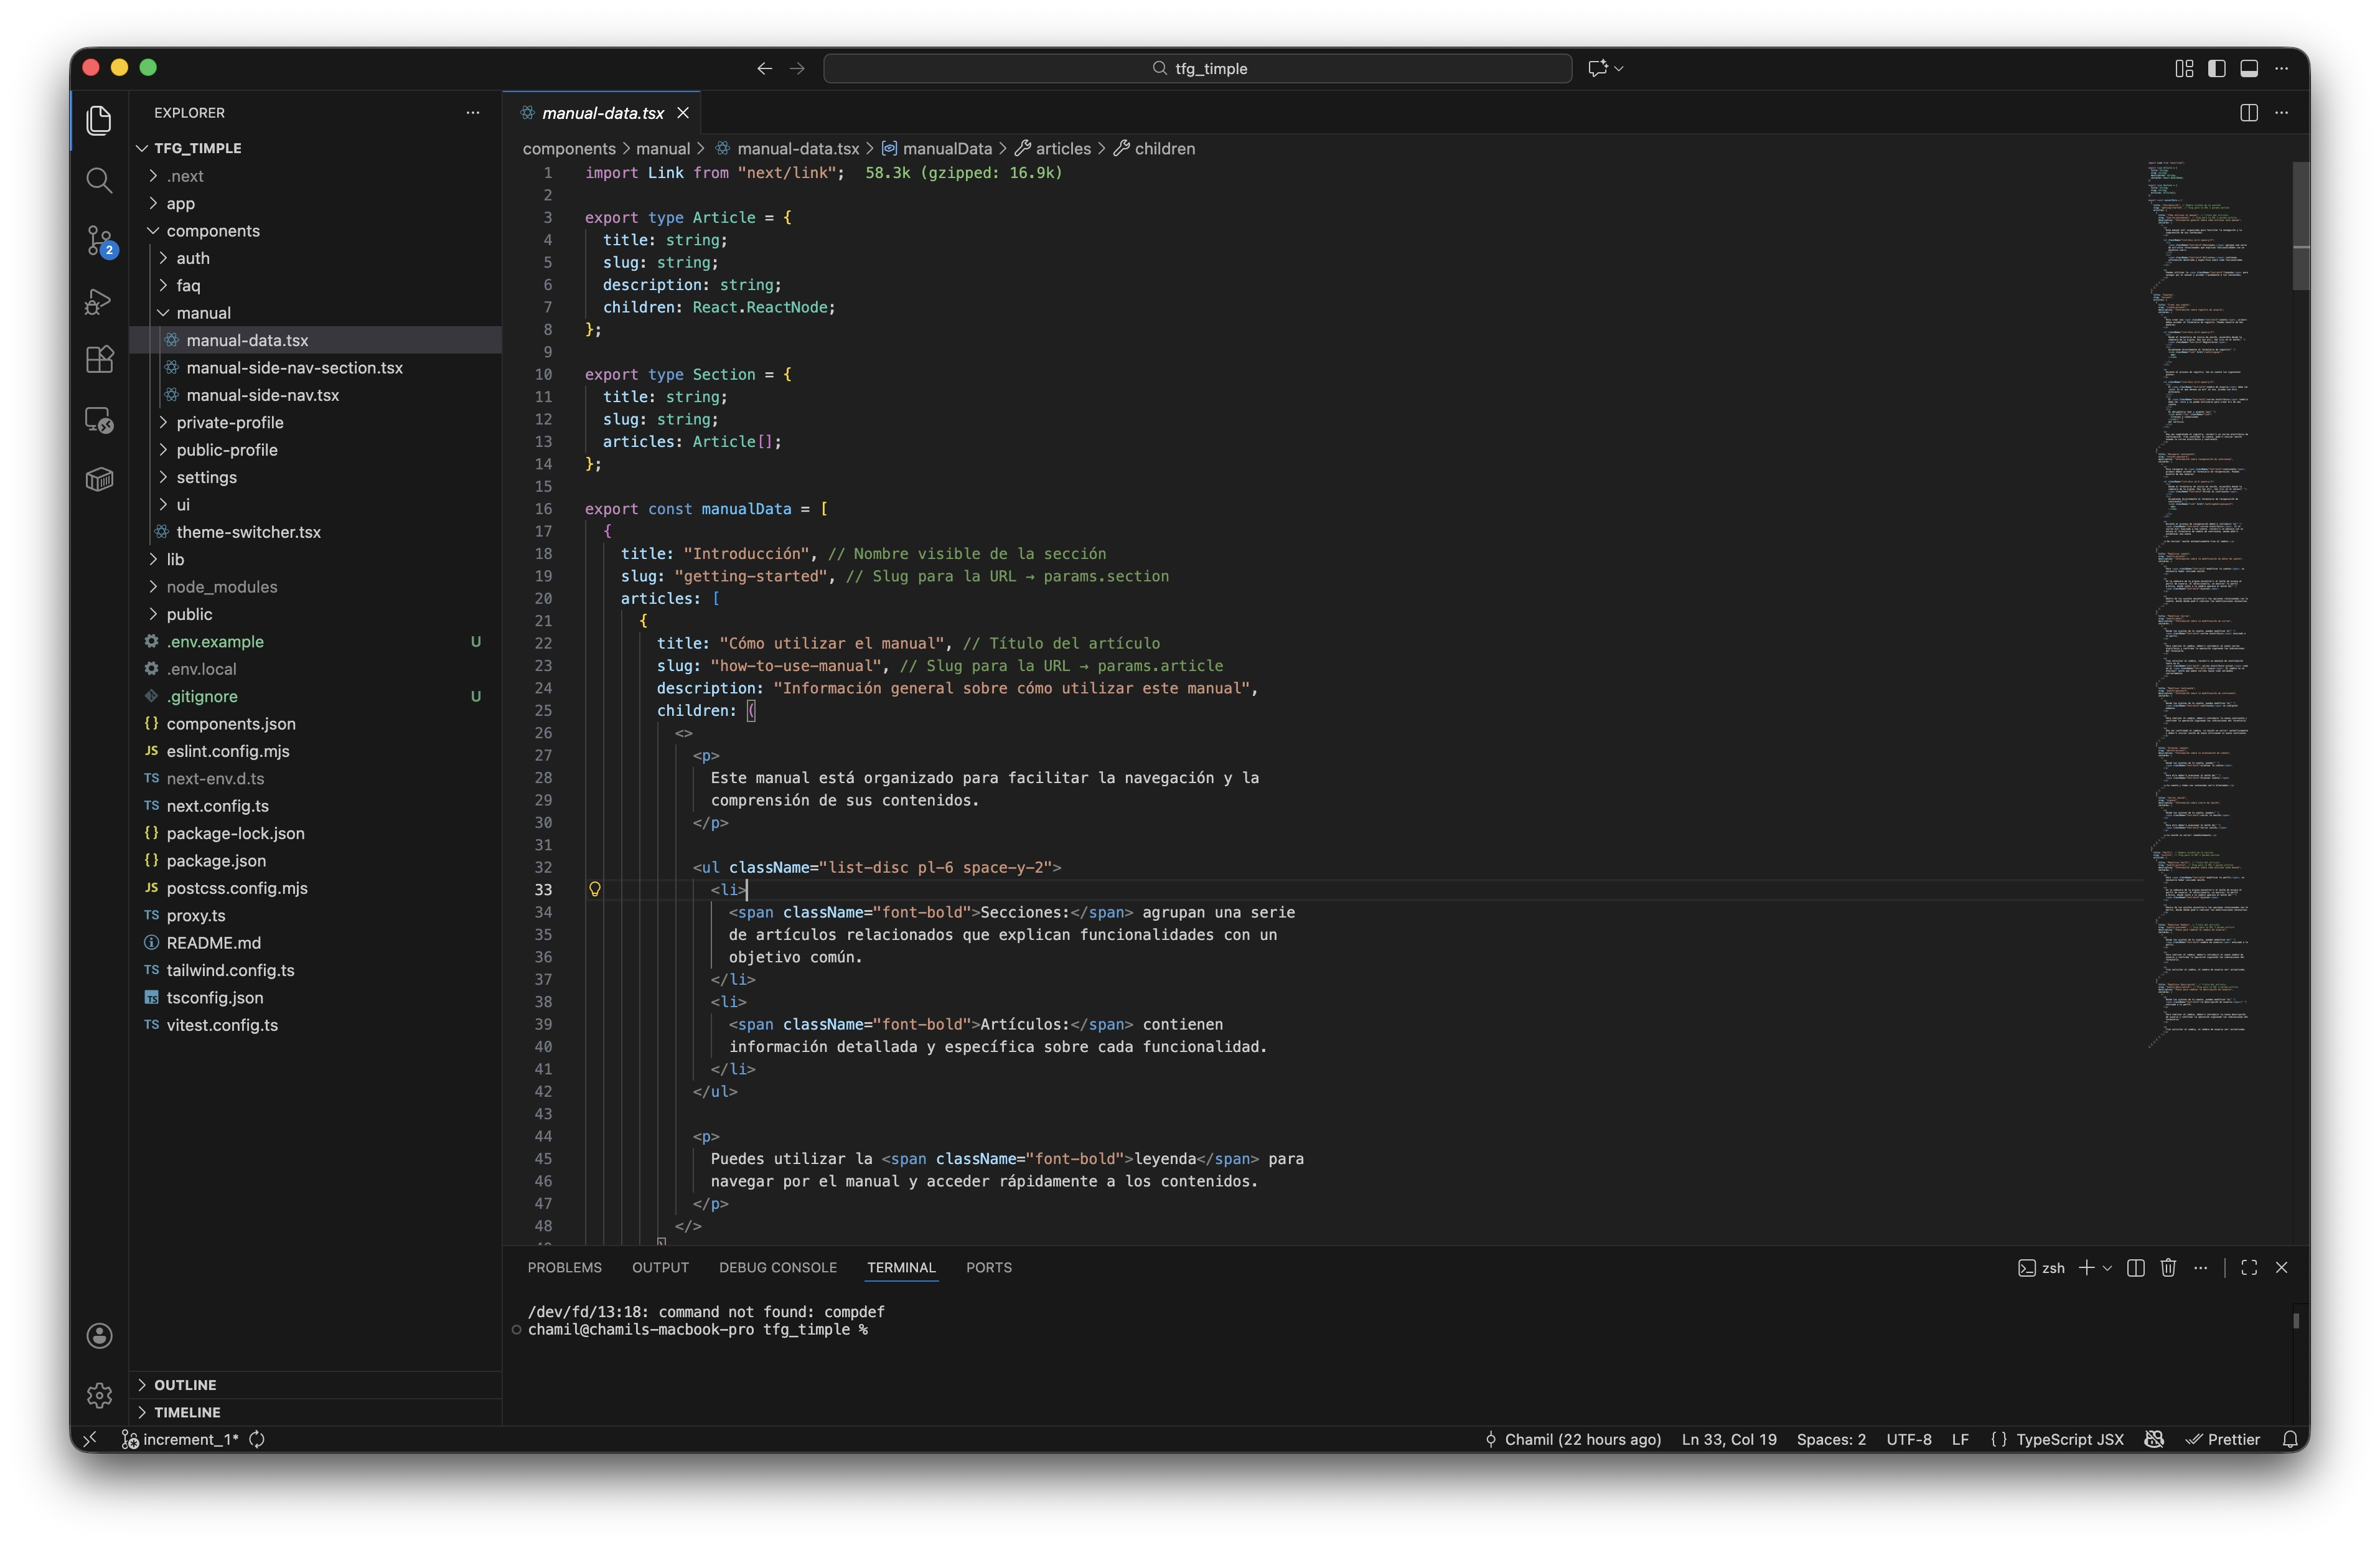
\includegraphics[width=0.8\textwidth]{Ilustraciones/desarrollo/incremento1/desarrollo/manual_it1.jpeg}
        \caption{Colección de información del manual de usuario}\label{fig:manual}
    \end{figure}

    \item Los \textbf{ajustes de cuenta} \figref{fig:dialogs}, donde se desarrollaron diálogos guiados por pasos, estableciendo un flujo estructurado de advertencia, modificación y confirmación del resultado.
    
    \begin{figure}[H]
        \centering
        \begin{subfigure}[t]{0.31\textwidth}
            \centering
            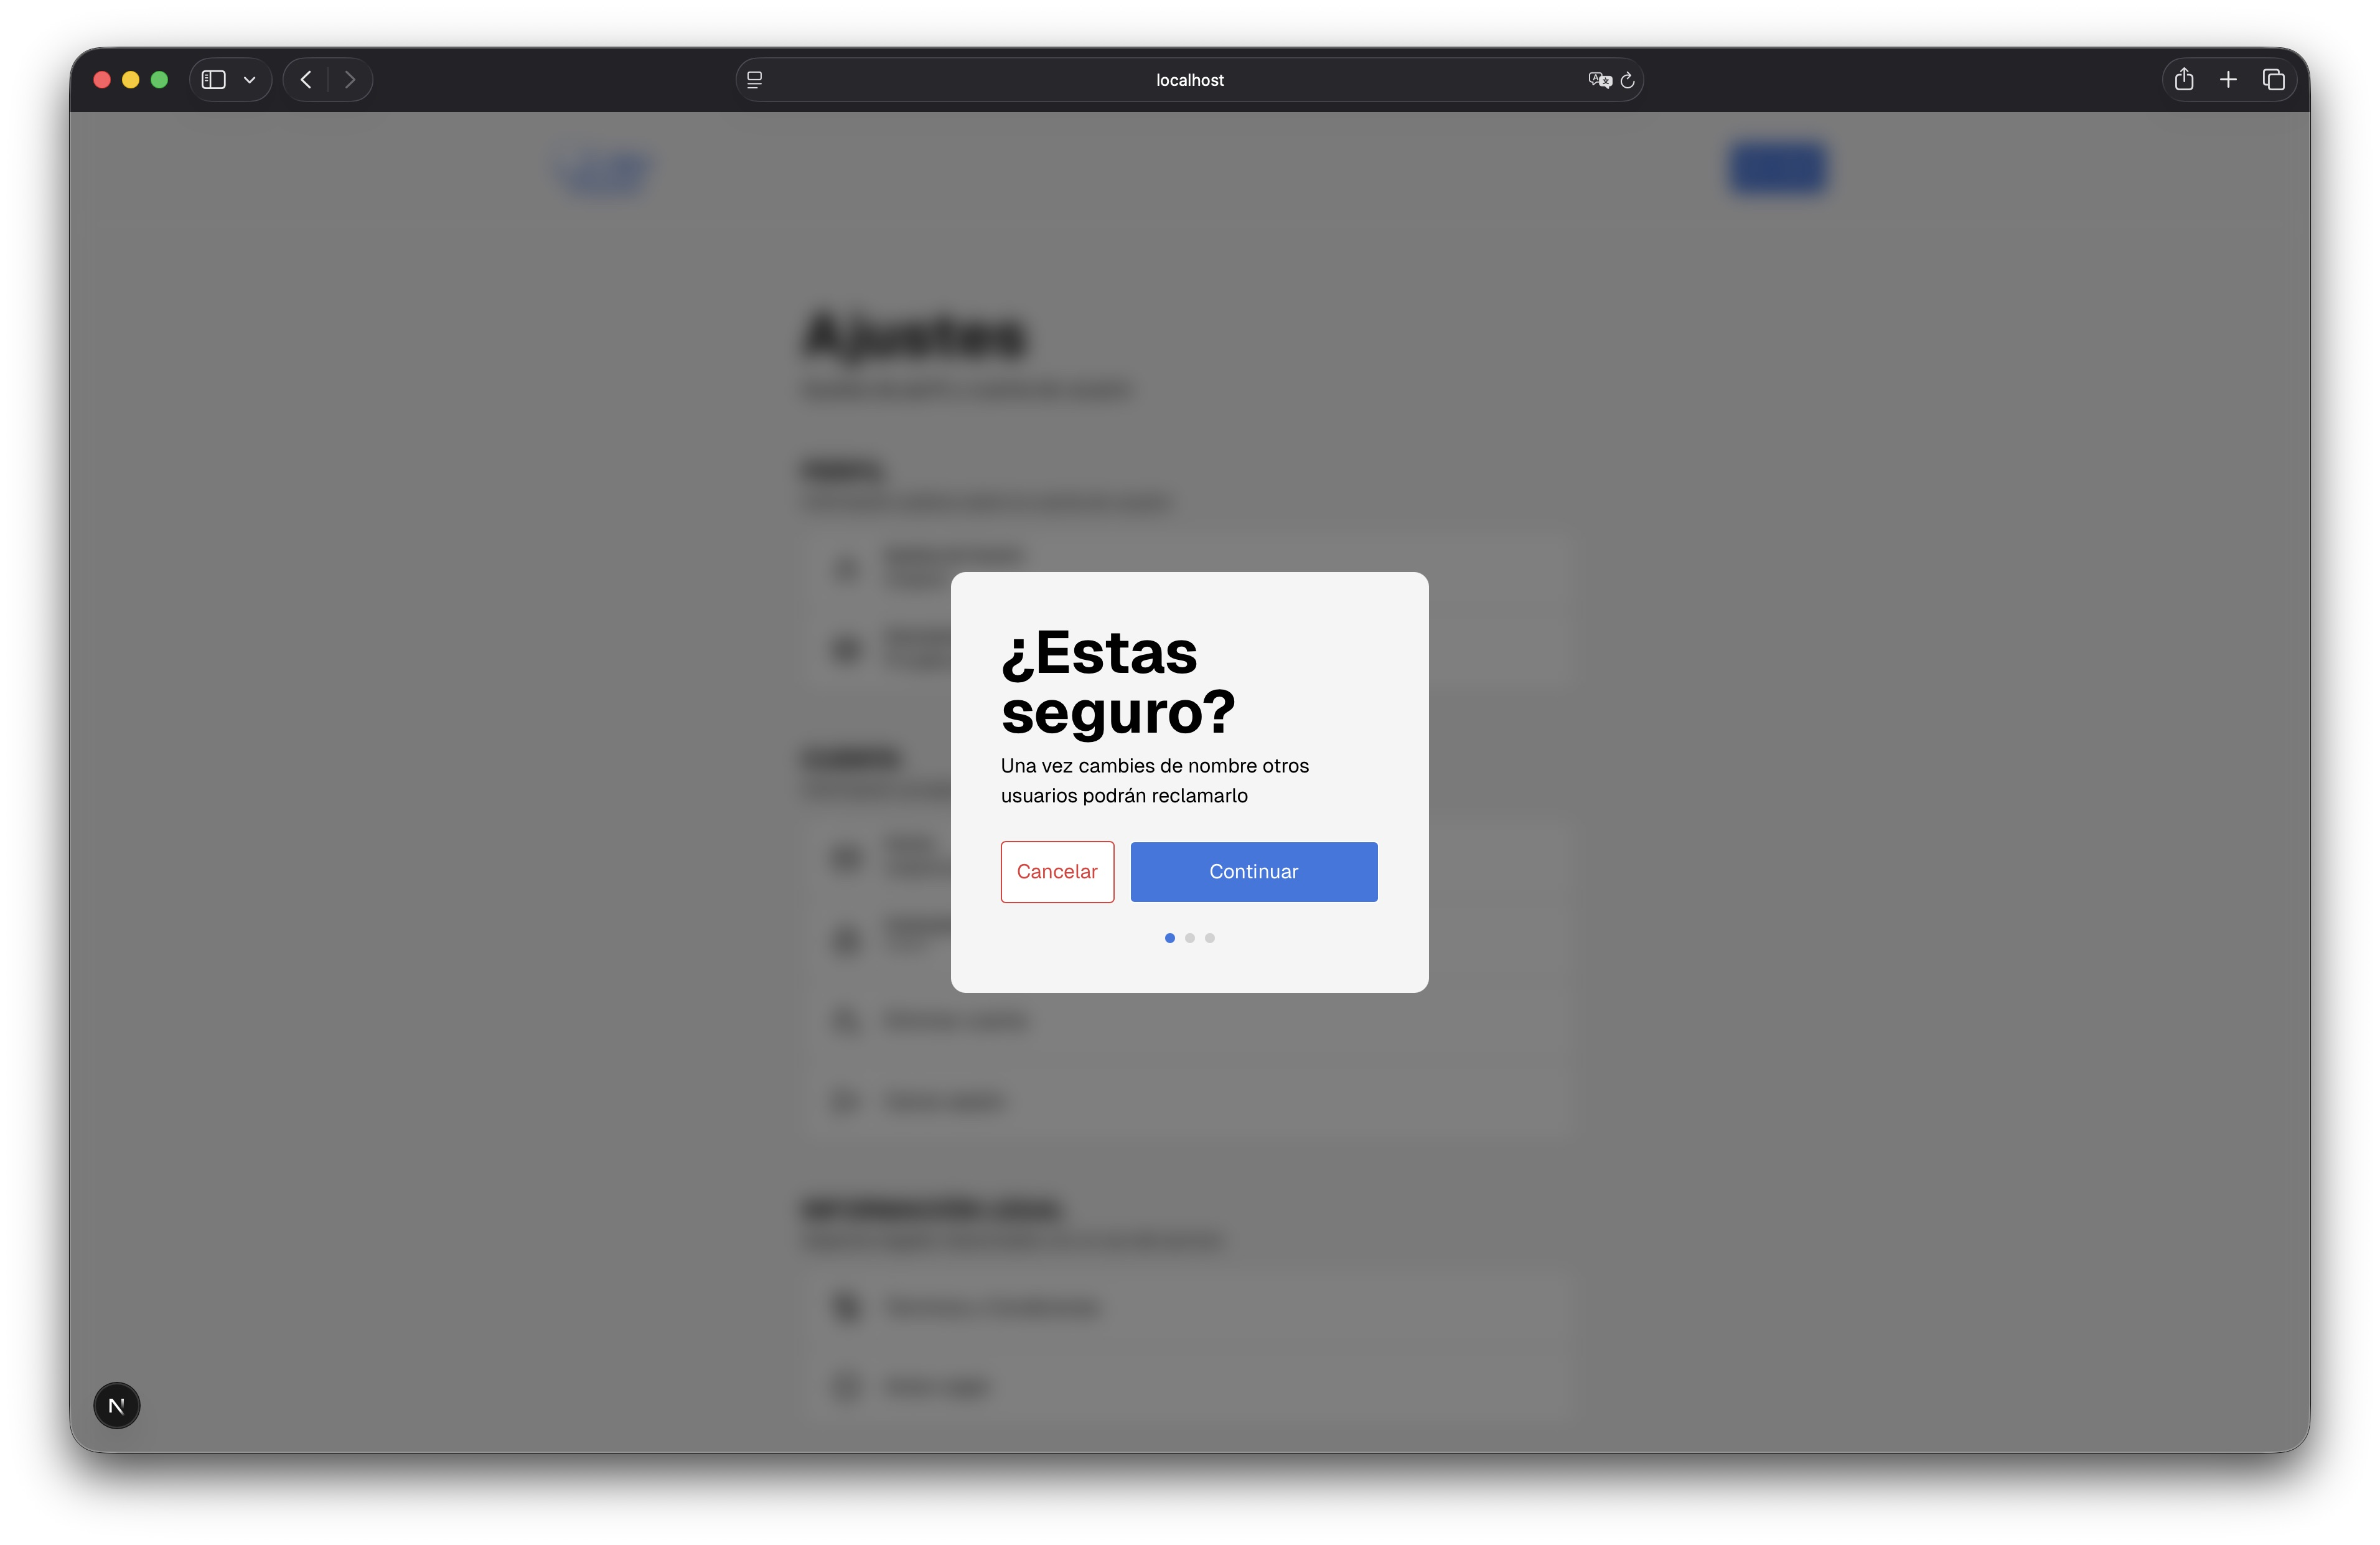
\includegraphics[width=\textwidth]{Ilustraciones/desarrollo/incremento1/desarrollo/dialog_1.jpeg}
            \caption{Dialogo de advertencia para la modificación de nombre de usuario}\label{fig:dialog_1}
        \end{subfigure}\hfill
        \begin{subfigure}[t]{0.31\textwidth}
            \centering
            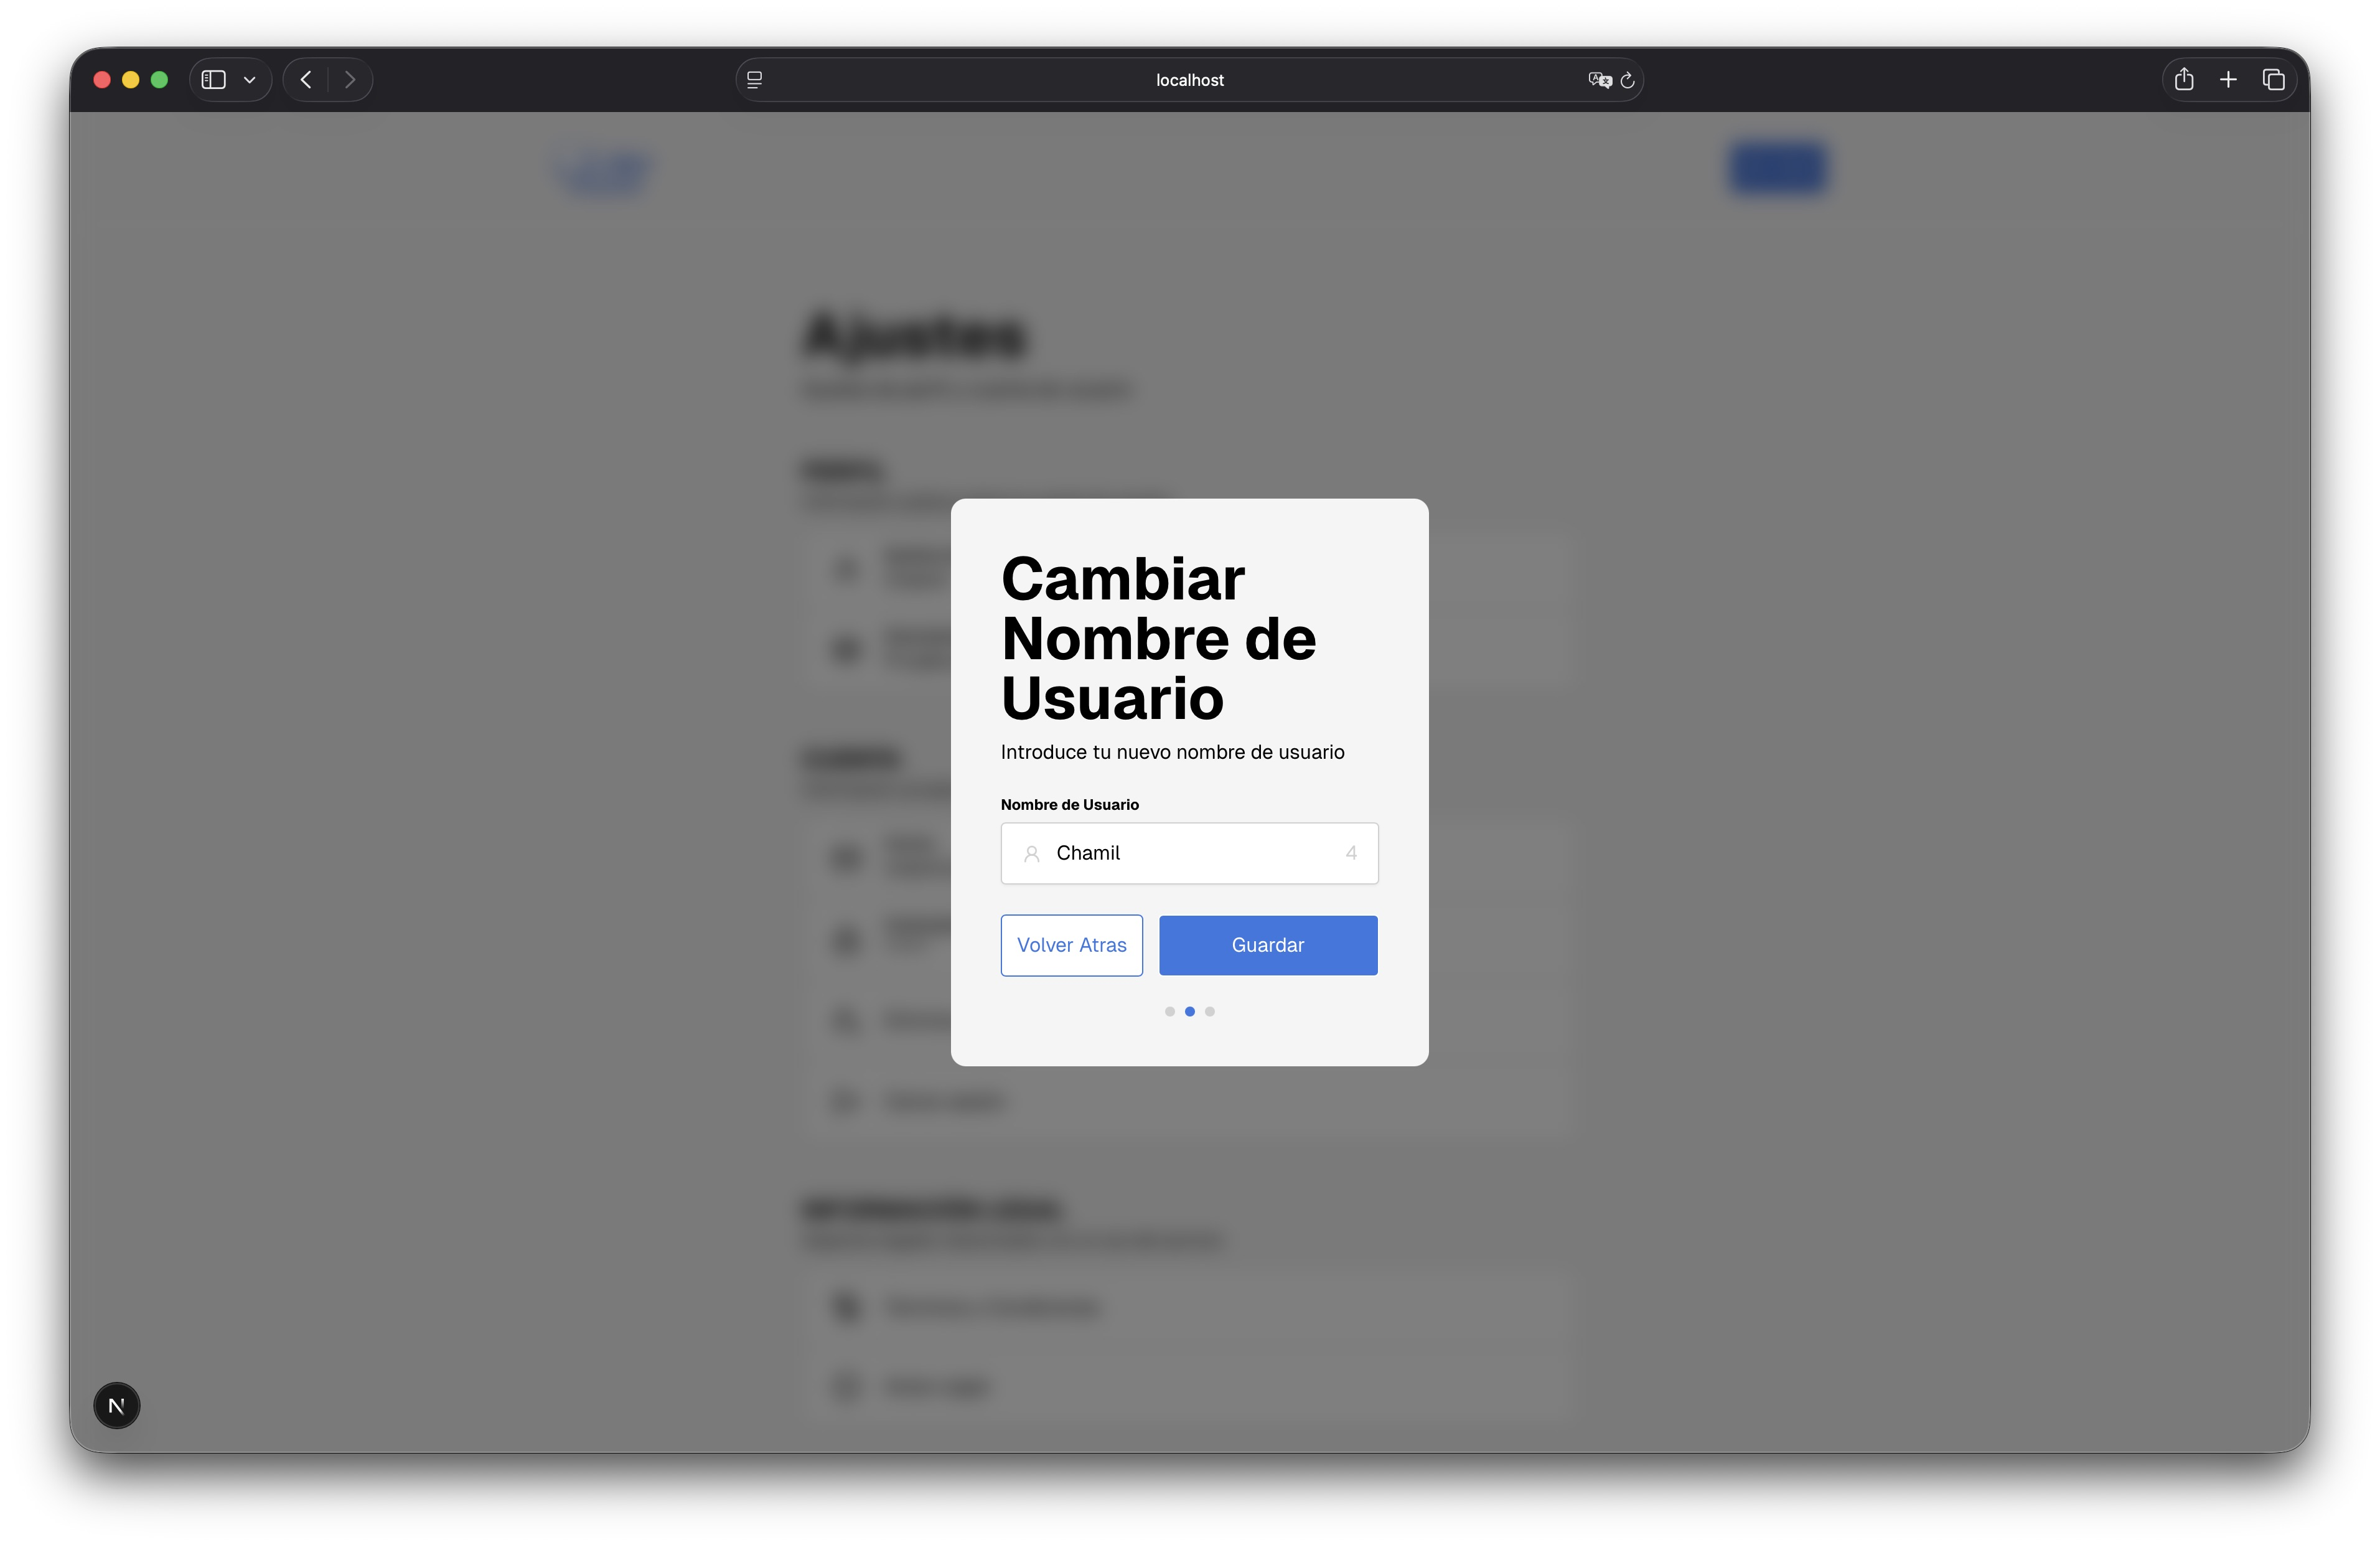
\includegraphics[width=\textwidth]{Ilustraciones/desarrollo/incremento1/desarrollo/dialog_2.jpeg}
            \caption{Dialogo de formulario para la modificacion de nombre de usuario}\label{fig:dialog_2}
        \end{subfigure}\hfill
        \begin{subfigure}[t]{0.31\textwidth}
            \centering
            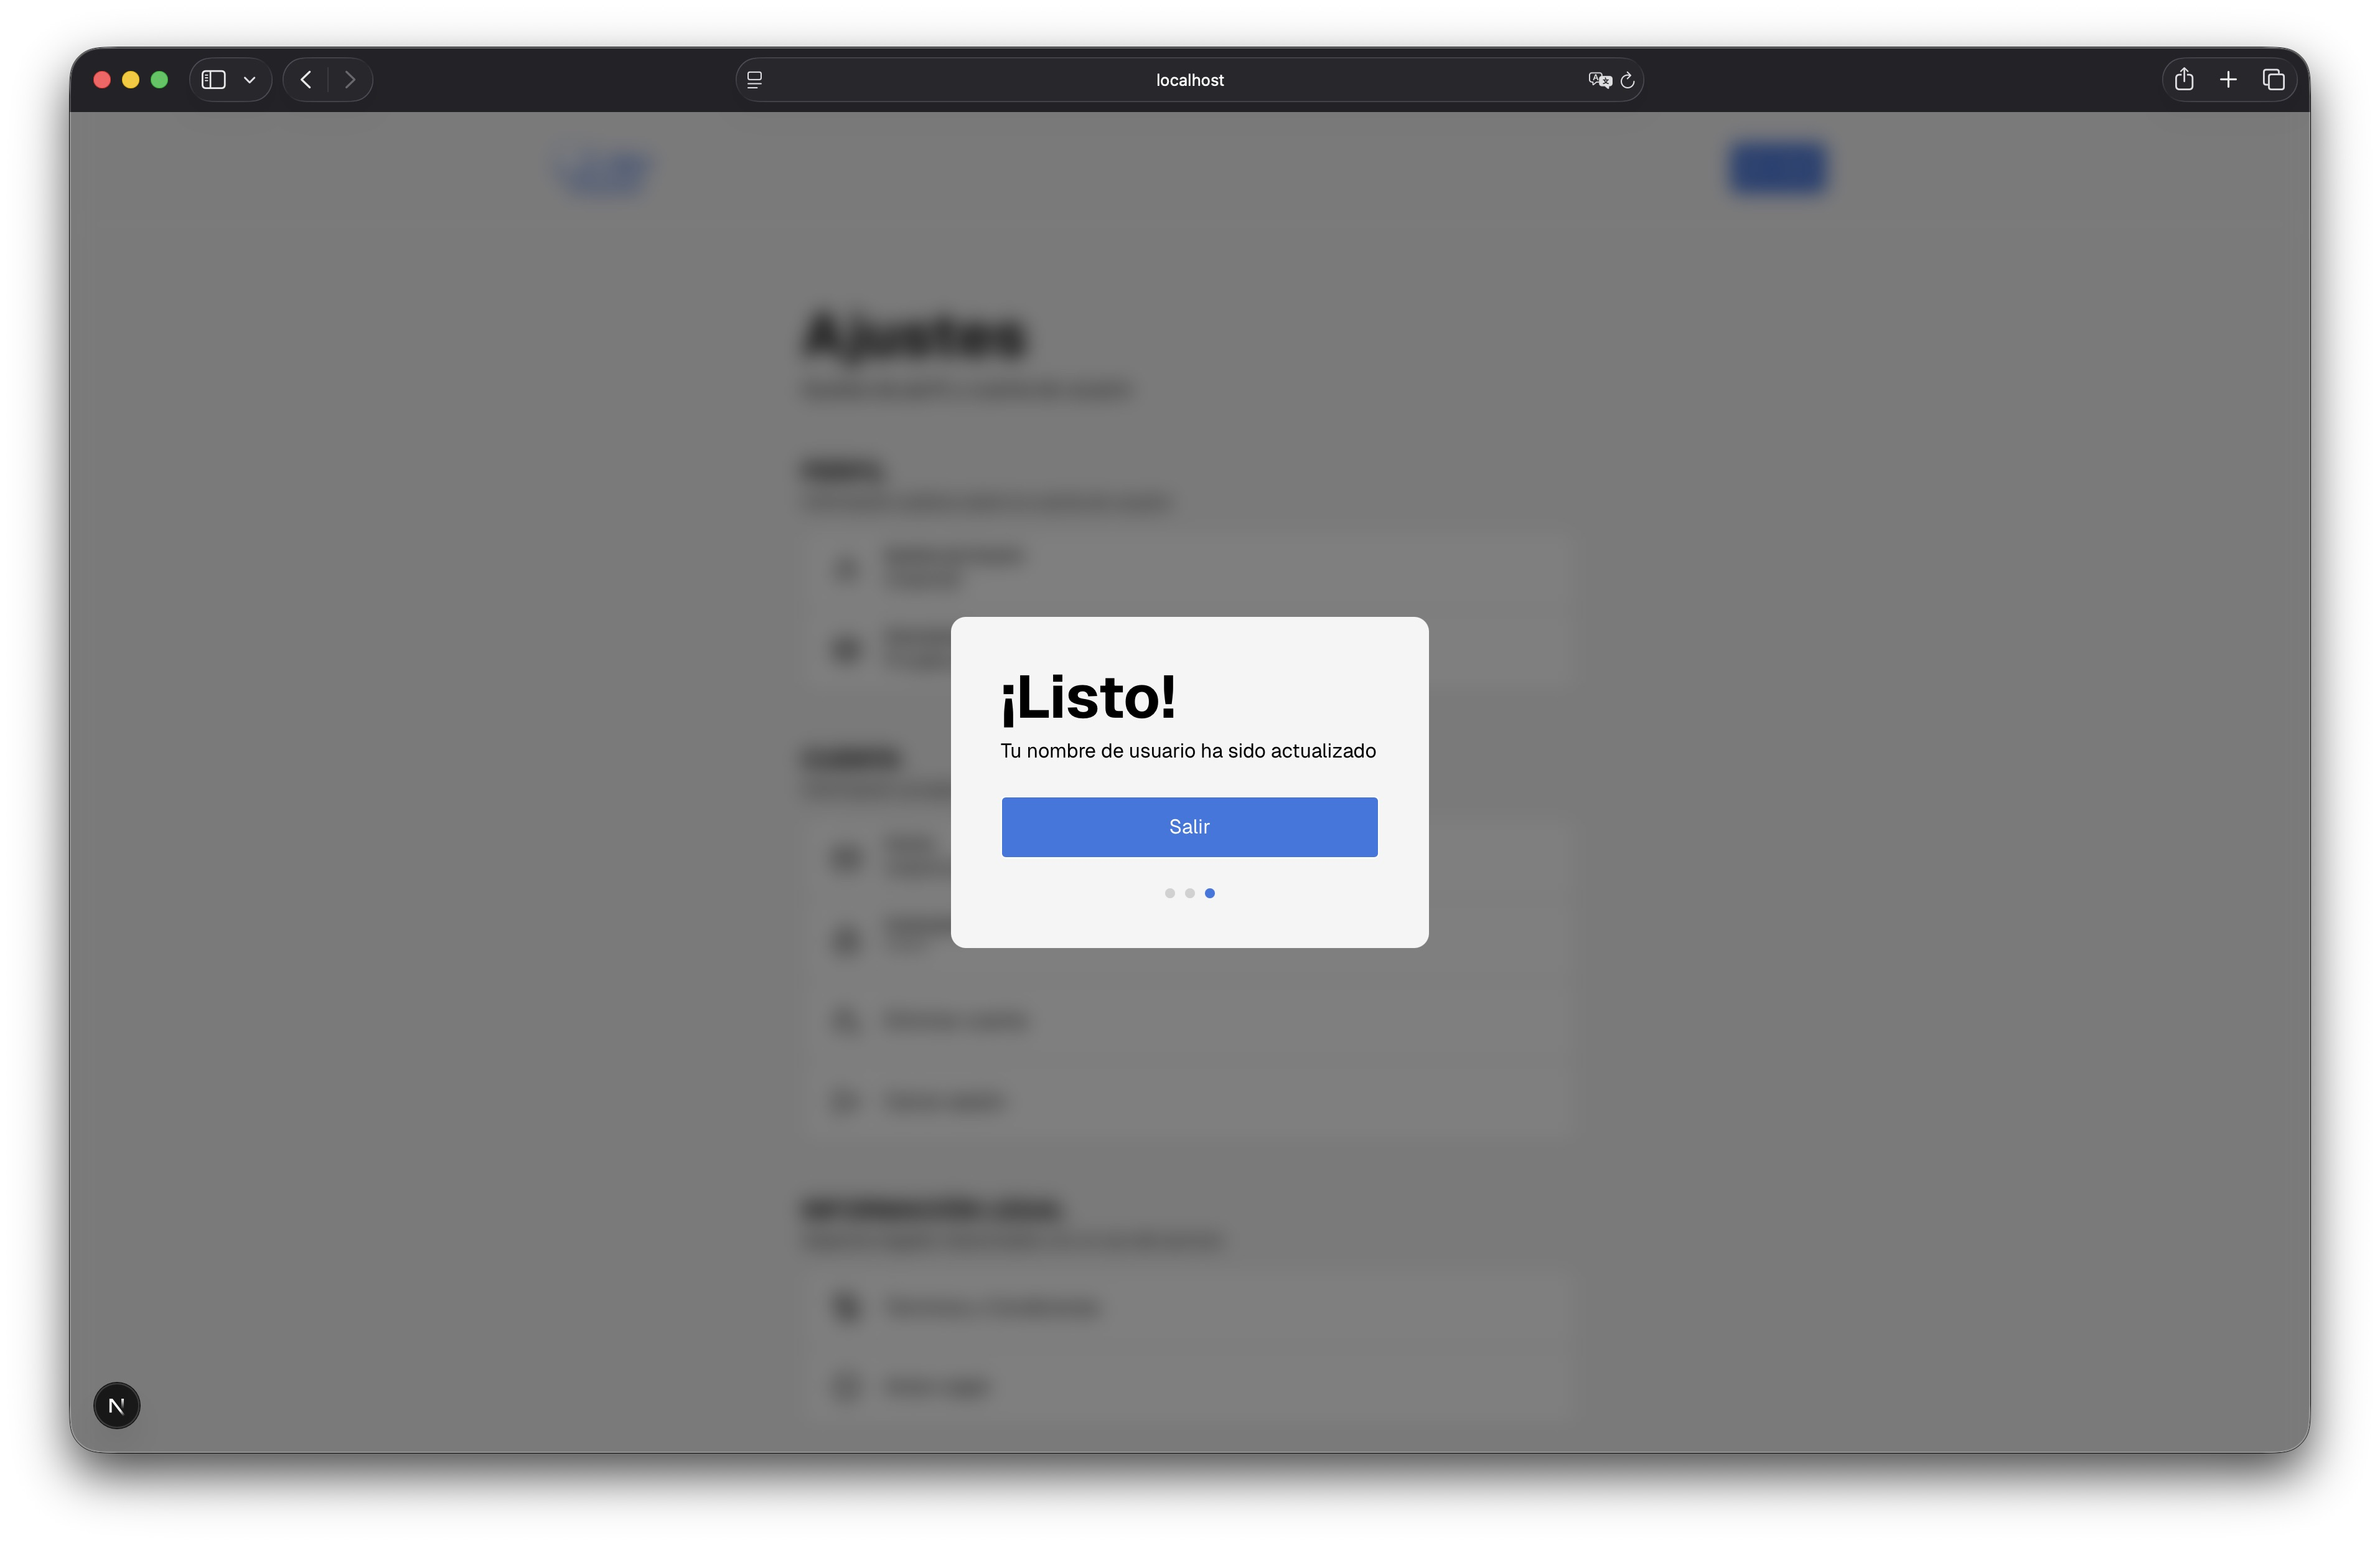
\includegraphics[width=\textwidth]{Ilustraciones/desarrollo/incremento1/desarrollo/dialog_3.jpeg}
            \caption{Dialogo de confirmación de cambio}\label{fig:dialog_3}
        \end{subfigure}
        
        
        \caption{Dialogos para la modificación de datos de cuenta}\label{fig:dialogs}
    \end{figure}

    \item Las páginas de \textbf{aviso legal} y \textbf{términos y condiciones}, en las que se redactaron los aspectos legales y las normas de uso del servicio.
    
    \begin{figure}[H]
        \centering
        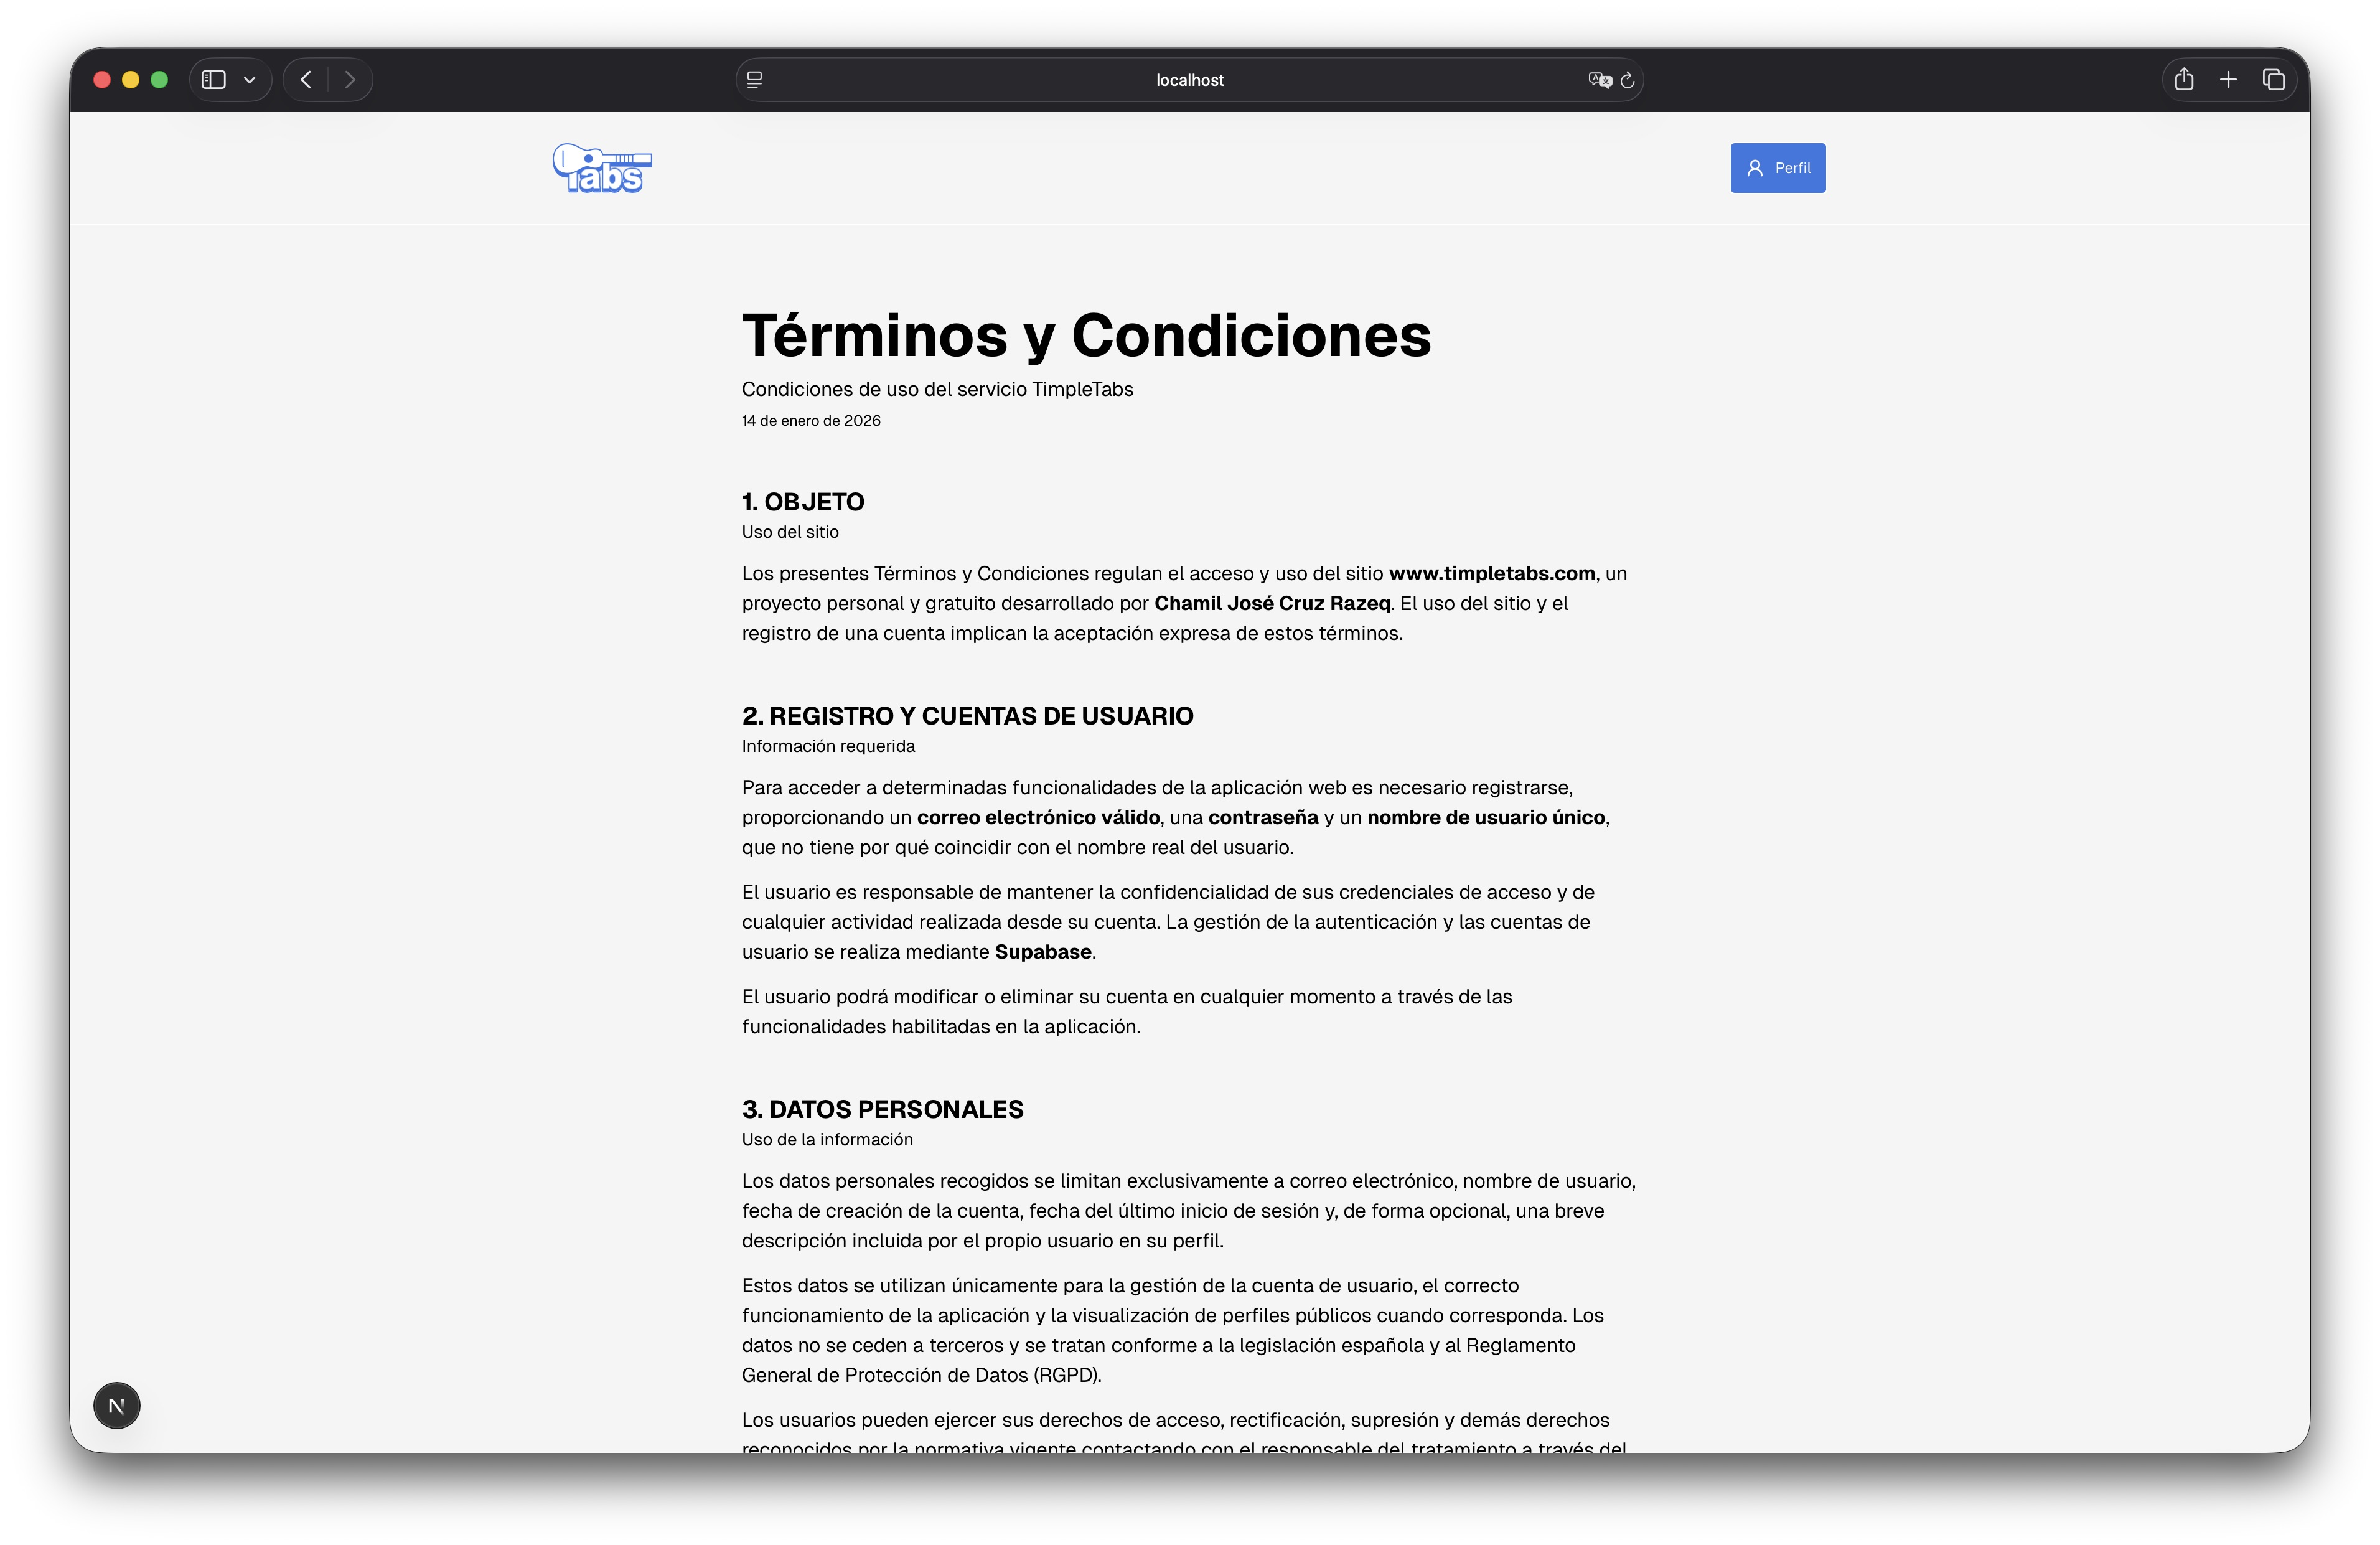
\includegraphics[width=0.8\textwidth]{Ilustraciones/desarrollo/incremento1/desarrollo/tac_it1.jpeg}
        \caption{Página de términos y condiciones del servicio}\label{fig:tac_it1}
    \end{figure}

\end{itemize}
